

\documentclass{svjour3}



\usepackage{comment}
\usepackage{listings}



\usepackage{url}
\usepackage{balance}

\usepackage{code}
\usepackage{graphicx}



% correct bad hyphenation here
\hyphenation{op-tical net-works semi-conduc-tor}

\journalname{Automated Software Engineering}

\begin{document}
\title{How Verified (or Tested) is My Code?\\Falsification-Driven
  Verification and Testing}

\author{Alex Groce \and Iftekhar Ahmed \and Carlos Jensen \and Paul
  E. McKenney \and Josie Holmes}

\institute{Alex Groce \at Northern Arizona University}

\begin{comment}
\author{\IEEEauthorblockN{Alex Groce, Iftekhar Ahmed, Carlos Jensen}
\IEEEauthorblockA{School of Electrical Engineering and Computer  Science\\
Oregon State University, Corvallis, Oregon\\
Email: agroce@gmail.com, ahmedi@onid.oregonstate.edu, cjensen@eecs.orst.edu}
\and
\IEEEauthorblockN{Paul E. McKenney}
\IEEEauthorblockA{IBM Linux Technology Center\\
Email: paulmck@linux.vnet.ibm.com}
}
\end{comment}


\maketitle


\begin{abstract}
Formal verification has finally advanced to a state where non-experts, including systems software developers, may want to verify the correctness of small but critical modules.  Unfortunately, despite considerable efforts in the area, determining if a ``verification'' actually verifies what the author intends it to is still difficult, even for model checking experts.  Previous approaches from the model checking community are valuable, but difficult to understand and limited in applicability.  Developers using a tool like a bounded model checker need verification coverage in terms of the software they are verifying, rather than in model checking terms.  In this paper we propose a tool framework and methodology to allow both developers and expert users to determine, more precisely, just what it is that they have verified for software systems.  Our basic approach is based on a novel variation of mutation analysis and a conceptual model of verification based on Popper's notion of falsification.  We use the popular C/C++ bounded model checker CBMC, modified to allow a user to determine the ``strength'' of a mutant, and show that this approach is applicable not only to simple (but complete, within bounds) verification of data structures and sorting routines, and verification of a routine in Mozilla's JavaScript engine, but to understanding an ongoing effort to verify the Linux kernel Read-Copy-Update mechanism.

\end{abstract}

\section{Introduction}


\begin{quote}
``Every `good' scientific theory is a prohibition: it forbids certain things to happen. The 
more a theory forbids, the better it is.''\\
-Popper, \emph{Conjectures and Refutations: The Growth of 
  Scientific Knowledge} \cite{popperconjectures}
\end{quote}

Software model checking \cite{ModelChecking} has recently, thanks to
improvements in model checking tools (and advanced SAT/SMT solvers), become
a potentially valuable tool for developers of critical software
modules who want to either perform a very aggressive search for
bugs or, ideally, prove correctness of their code.  Tools such as
CBMC \cite{CBMCp} (the C Bounded Model Checker) allow a software
engineer to model check code by writing what is essentially a
generalized test harness \cite{woda12,woda08}\footnote{By a harness we mean a program that
  defines an environment and the form of valid tests, and provides
  correctness properties.} in the language of the Software Under Test
(SUT).  Figure \ref{fig:sortharness} shows an example CBMC harness for
sorting routines.  Only a few aspects differ from normal testing.
First, {\tt nondet\_int} in CBMC can return any value.  It is
not equivalent to a ``random'' choice but true nondeterminism: CBMC
will explore all values of the type.  The {\tt \_\_CPROVER\_assume}
statement has the usual
{\tt assume} semantics \cite{EWD:Discipline,exploit}: CBMC ignores
all executions that violate assumptions.

\begin{figure}
{%\scriptsize
\begin{code}
\#include "sort.h"

int a[SIZE];
int ref[SIZE];

int nondet\_int();

int main () \{
  int i, v, prev;
  int s = nondet\_int();
  \_\_CPROVER\_assume((s > 0) \&\& (s <=SIZE));
  for (i = 0; i < s; i++) \{
    v = nondet\_int();
    printf ("LOG: ref[\%d] = \%d\\n", i, v);
    ref[i] = v; a[i] = v;
  \}
  sort(a, s);
  prev = a[0];
  for (i = 0; i < s; i++) \{
    printf ("LOG: a[\%d] = \%d\\n", i, a[i]);
    assert (a[i] >= prev);
    prev = a[i];
  \}
\}
\end{code}
}
\caption{CBMC harness to check a sorting routine.}
\label{fig:sortharness}
\end{figure}

CBMC compiles a harness and the SUT (here a quicksort implementation)
into a goto-program, instruments this program with property checks for
assertions, array bounds violations, etc., and then unrolls loops
based on a user-provided unwinding bound to produce a SAT
problem or SMT constraint such that satisfying assignments are
representations of a trace demonstrating a property violation, known
as a counterexample \cite{CountWitness}.  For CBMC, this means
that if \emph{any possible execution allowed by the harness} violates
any properties checked, a counterexample will be produced.  This
includes user-specified assertions and automatically generated
properties such as array bounds and pointer validity checks. One
generated property is that no loop in the program executes more than
the \emph{unwinding bound} times.  For example, if we run CBMC on the
harness shown and set the unwinding bound to 3 and add {\tt -DSIZE=2},
we will check the correctness of the SUT over all possible
  arrays of size 2 or less, including checking that sorting never
requires passing through any loop more than 3 times.

When a model checker produces a counterexample, a developer's task is
straightforward, if sometimes difficult: either the SUT has a fault,
or the harness itself is flawed.  In both cases, the output of the
verification effort is the counterexample trace, which is full of
evidence as to the reason for the failure to verify the SUT. Moreover,
any solution (fix to SUT or harness) is easily checked: if it is
correct, the model checker stops reporting the previous
counterexample.  
This is essentially a normal debugging problem, but
with the advantage that solutions are easily checked.

Unfortunately, model checkers do not invariably report
counterexamples: eventually the SUT is likely to satisfy the
properties encoded in the harness!  It is in this case that problems
arise: what, precisely, has been verified?  Is the SUT actually correct?
Formal verification is not only subject to the problems that make
``no faults detected'' results dubious in testing \cite{WODA09,CovDisc}, but
also to more subtle problems.  For example, an incorrect {\tt assume}
statement may constrain a system so that not only are there no
counterexamples, there are no (interesting) executions of the system at
all.  Moreover, formal verification tools are themselves extremely
complex software artifacts, and, like production compilers \cite{csmith}, may
themselves have serious bugs that produce wrong results
\cite{statanalbug}.  In the course of this research, we have ourselves
encountered several tool-induced incorrect verifications.

The problem of checking verification results has concerned the model checking community for some time, and resulted in efforts to define \emph{coverage
  metrics} for model checking \cite{Hoskote,PracticalCov}.  While such metrics are interesting and
useful, they have typically been aimed at hardware
verification, and most useful to experts in
formal verification.  In this paper, we adapt traditional mutation
testing \cite{mutation1,mutation2} to the problem of software
verification.  A mutant of a program is a version of the program with
a small syntactic change.  The idea behind mutation testing
is that a good test suite will be able to detect when (as is usually
the case) such a change introduces a bug in the SUT.  In the case of
bounded model checking, since we aim at (bounded) verification rather
than merely good testing, surviving mutants are
likely to indicate a real problem.

In software engineering research, mutation is often used only as a way
to compare competing test suites by comparing kill rates \cite{ISSTA13,TOSEM14}.  This is
not enough for verification.  The typically small scope of the code to
be verified, and the presumed importance of verified code
suggests an approach in which \emph{individual mutants}
are examined by the developer.  Without additional assistance, such an
approach cannot scale.  This paper aims to describe how to make this
seemingly too-demanding approach practical for real verification
tasks.


Our basic idea is to use mutants \emph{throughout the verification
  effort}, even in choosing a bound for bounded model checking.  At
each stage the developer examines the currently surviving mutants,
either by inspecting the mutated code or (when this does not make the
reason the mutant is not detected clear) looking at \emph{successful
  executions covering the mutant but satisfying the specification
  given in the harness}.  For critical verification tasks, we suggest
that developers not only examine the passing executions of surviving
mutants, but the passing executions of \emph{killed mutants}.  While
examining test cases that do not kill a given mutant could be useful
in traditional testing, the model checker makes a much more potent
investigation possible, where a developer can constrain the behavior
to force the mutant's behavior to matter, if that is possible, and
automatically find passing executions that maximize coverage
(including the mutated code).  We also propose that a developer should
use mutants of the test harness itself to ensure that no similar
harness has a better mutant kill rate, and that most mutants of the
harness reject the SUT itself.

\subsection{Contributions}

This paper is an extension of a paper presented at the 30th IEEE/ACM
International Conference on Automated Software Engineering in 2015
\cite{ase15}.  
The core contribution of that earlier paper was a \emph{falsification-driven}
verification methodology using mutants to aid developers 
 in understanding ``successful'' verification
results, determining when a harness is flawed, and correcting the harness.
It showed how to use mutation testing to
choose a problem size in bounded model checking, how to mutate a
harness to determine if any similar harnesses have an equal (or
better) mutation kill rate, and most importantly, how to modify CBMC,
a harness, and mutants to automatically produce successful
 high-coverage executions covering mutated code in order to
understand mutant (and thus harness) behavior.  This
approach, unlike a simpler method of searching for cases where the
mutated and original code behave differently for identical inputs,
in principle applied to verification of reactive and concurrent systems, where
there is no simple notion of identical inputs.  
It also proposed the use of mutation analysis to gain limited confidence
in program correctness even past model checker scalability limits. 
At a more general level, the original paper discussed the fundamental nature of
``verification'' in a real-world context where specifications are
never known to be complete.  The central concept of that paper, and
this extension, is that falsification, as in Karl
Popper's famous philosophy of scientific discovery \cite{Popper}, is
the critical element of efforts to understand systems, efforts that are always
provisional by nature:  e.g., most program verification (and even more
so, testing) efforts.  Popper's approach therefore forms a 
useful conceptual
framework for verification efforts: rather than focusing on what can
be proven about a program, we propose that correctness-determination efforts focus on how a
verification distinguishes the ``real'' program from similar
alternative programs that do \emph{not} match the theory of program
behavior.  Such an approach still aims at verification as a final outcome, but continually
evaluates and refines that verification effort by its ability to
\emph{falsify} rather than to verify.

In this paper, we extend the contributions of the previous work by
further elaborating the approach to bounded model checking presented
there, but, most significantly, we extend the same ideas to automated
software testing, where there are new challenges and it is less clear
that the underlying concepts are sound.  In our previous work, we
dismissed the possibility of using our approach for testing, because
when a typical test generation approach fails to find a failing test
(that is, testing's version of a counterexample), it does not mean the
property is insufficient, or even that the generation is weak.
Testing is usually essentially probabilistic.  Here we show that this
limitation is not fundamental, and the same principles can apply to
serious automated test generation efforts as well.  The general ideas
are analogous, including the modification of a test generation tool to
generate high-coverage tests that 1) fail to kill a mutant but 2)
cover the mutated code, in order to facilitate understanding of the
limits of a harness, but the details require considerable modification
in order to adapt to the probabilistic context of test generation.
For example, the equivalent of a problem size for bounded model
checking is a test budget for automated test generation; however,
rather than a fixed outcome, the problem in this case is to present a
likelihood curve to users, and allow them to make tradeoffs based on
that curve.

We still initially present our approach in the context of formal
verification, where it is most obviously useful, and where there is a
higher chance of killing enough mutants to make manual analysis of
un-killed mutants feasible.

\section{A Simple Example Verification}

\begin{figure}
{%\scriptsize
\begin{code}
 \#include "sort.h"

 void quickSort( int a[], int l, int r)
 \{

   printf ("LOG: called with l=\%d, r=\%d\\n", l, r); 
   int j;

{$_9$}  if( l < r ) 
     \{
       // divide and conquer
       j = partition( a, l, r);
       quickSort( a, l, j-1);
       quickSort( a, j+1, r);
     \}
  
 \}

 int partition( int a[], int l, int r) \{
   int pivot, i, j, t;
   pivot = a[l];
   i = l; j = r+1;
  
{$_{26}$} while( 1)
     \{
{$_{28}$}     do ++i; while( i <= r \&\& a[i] <= pivot );
       do --j; while( a[j] > pivot );
{$_{30}$}     if( i >= j ) break;
{$_{31}$}     t = a[i]; a[i] = a[j]; a[j] = t;
     \}
   t = a[l]; a[l] = a[j]; a[j] = t;
   return j;
 \}


 void sort(int a[], unsigned int size) \{
   quickSort(a, 0, size-1);
 \}
\end{code}
}
\caption{Quicksort code.}
\label{fig:qsort}
\end{figure}

As an example of the proposed verification methodology, consider again
the harness shown in Figure \ref{fig:sortharness}.  If we take an
early Google result for ``quicksort in C'' \cite{quicksortcode},
shown in Figure \ref{fig:qsort}\footnote{In fact, that actual code is
  incorrect, with an access {\tt a[i]} that does not properly use
  short circuiting logical operators to protect array bounds; CBMC
  detected this, and we fixed it for this paper.}, we can model check
it using the harness, defining {\tt SIZE=2} and setting the unwinding
bound to 3 (we need one more unwinding than the maximum
number of items in the array).  CBMC reports {\tt VERIFICATION
  SUCCESSFUL} in less than a second.  Have we verified
what we want to verify?

\subsection{Finding a Good Problem Size}
\label{sec:unwind}

The first question we face is whether 2 is a good maximum array
size to examine.  The problem of determining a completeness
  threshold (an execution-length bound sufficient to prove correctness
in all cases for a given property) for bounded model checking is
fundamentally difficult \cite{CTDaniel} and is, for real-world C
programs, more an art than a science at present\footnote{In our own
  practice, the most common way of setting it is to guess a bound and
  see if the resulting problem is too large for the available
  resources.}.  Are there bugs for which 2 is too small
an array size?  In order to find out, we generate a set of mutants for
{\tt quicksort.c}.  Using the mutation tool for C code developed by
Jamie Andrews \cite{mutant}, we can produce 81 mutants of this code in
less than a second.  We then run the harness with unwinding bound 2
(and {\tt SIZE=1}) on each of the 81 mutants.  The process takes less
than a minute and a half (on a MacBook Pro with 16GB RAM and dual-core 3.1GHz Intel
Core i7, using only one core).  CBMC reports that 6 mutants do not
compile (these remove variable declarations, for the most part), 4 are
detected by the harness (a counterexample is produced: we say the
mutant is killed), and 71 mutants pass without detection (the
verification is successful, in which case we say the mutant survives).
Clearly length 1 arrays are not sufficient to detect even the most
glaring bugs in a sort algorithm (no surprise: all size 1 arrays are
sorted).  What about our choice of size 2?  Re-checking the mutants
with this bound
(dropping those already killed by the smaller bound) takes slightly
over 13 minutes (due to one mutant requiring over 8 minutes
to model check) and reduces the number of surviving mutants to 26.  We
could inspect these mutants by hand, but it seems highly unlikely that
a complete verification over all possible arrays with a good
specification for sorting would produce such a poor mutation kill rate.
If we increase the size limit to 3 and unwinding 4 (now the analysis takes just over 33
minutes), only 8 mutants survive.  Note that each problem, due to the
harness' assignment of {\tt s} to any size smaller than the current
size, includes all smaller problem sizes. This makes the behavior of
the verification problem size setting match that of CBMC where an unwinding bound is a maximum, rather than
a fixed size.  We assume inclusiveness in this paper\footnote{There is
  one noted exception in Section \ref{sec:sattimes}.}.

At this point, we can increase {\tt SIZE} to 4 (which will kill one
additional mutant), but the time required to check the remaining
mutants is growing rapidly.  In fact, completing the check for size 4,
even though only the original program and 8 mutants have to be
checked, requires nearly 9 hours.  When the model checking
difficulty grows more slowly with problem size, we propose the simple
(if highly imprecise)
heuristic of increasing
size until the number of mutants killed does not increase with a step
up in size (we call such a size
\emph{mutant-stable}).  However, in
many cases, such as this one, the time required to check mutants
starts growing unacceptably.  We propose a more efficient algorithm
for finding a mutant-stable size below (Figure \ref{alg:unwind}), and
mutations can be checked in parallel, but the fundamental problem for
size 4 (and above) is that some individual mutants require hours to
model check.  What is a developer to do?


\subsection{Examining Surviving Mutants}
\label{sec:maxcover}


\begin{figure}
{%\scriptsize
\begin{code}
 9 :   /*(rep\_op)*/ if (l <= r) 
 26 :  /*(rep\_const)*/ while(-1)
 26 :  /*(rep\_const)*/ while( ((1)+1))
 28 :  /*(rep\_op)*/ do ++i; while(i<r \&\& a[i]<=pivot);
 28 :  /*(rep\_op)*/ do ++i; while(i!=r \&\& a[i]<=pivot);
 28 :  /*(rep\_op)*/ do ++i; while(i<=r \&\& a[i]<pivot);
 30 :  /*(rep\_op)*/ if( i > j ) break;
 31 :  /*(del\_stmt)*/ t=a[i]; /*  a[i]=a[j]; */  a[j]=t;
\end{code}
}
\caption{Surviving mutants at {\tt SIZE=3}.}
\label{fig:survivors}
\end{figure}

The developer should turn to the surviving mutants.  The 8 surviving  
mutants for size 3 are shown in Figure \ref{fig:survivors}.  
The comment indicates the type of mutant, and the line number in the quicksort file is also given for reference.  The relevant lines are marked
in Figure \ref{fig:qsort}.  Some of these mutants are easily seen to
be equivalent to the original code.  For example, the two {\tt
  rep\_const} mutations simply change a {\tt while(1)} into an
equivalent infinite loop with a different constant non-zero value.
These two mutants could in fact have been automatically removed from
the set, like uncompilable mutants, by checking their compiled code
for equivalence with the original program \cite{TCE}.  We suggest
always pruning mutants via Trivial Compiler Equivalence (TCE).  The remaining 6 mutants produce different
binaries when compiled with an optimizing compiler, so require manual
analysis.  The 5 {\tt rep\_op} mutations all alter comparison
operators by changing their value on one corner case, and we may suspect that quicksort is robust to,
for example, changing {\tt i <= r} to {\tt i != r} since {\tt i} is
initially set to {\tt l}, which we know to be less than {\tt r}.

The {\tt del\_stmt} mutant, however, is clearly problematic.  How can
quicksort be correct if the inner loop's swapping of {\tt a[i]} and
{\tt a[j]} is changed to instead copy {\tt a[i]} to {\tt a[j]}?  The
consequences of this mutant are clearly drastic, but why are they not
detected by our harness?  We find out by asking CBMC to produce an
execution such that 1) the mutated code is covered 2) other coverage
is maximized (to avoid degenerate executions, e.g., over size 1
arrays) and 3) the execution is not a counterexample.  We have
modified CBMC, and written instrumentation tools that produce a
modified mutant and harness, allowing us to pose such queries (see
Section \ref{sec:algs}).  Running CBMC in this mode, with the target of maximum branch
coverage and statement coverage of the {\tt del\_stmt} mutant
(actually the statement after it, since it no longer exists),
we produce the witness in Figure \ref{fig:witness1} in less
than a minute\footnote{We show the output of the print statements, not
  the full CBMC trace: this is what a developer will examine first.}.  Our harness
checks that the array {\tt a} is sorted after the call to {\tt
  sort}, but it does not check that it is a permutation of the input!

\begin{figure}
{%\scriptsize
\begin{code}
LOG: ref[0] = 2147414872
LOG: ref[1] = 2147480408
LOG: ref[2] = -1073743560
LOG: called with l=0, r=2
LOG: called with l=0, r=-1
LOG: called with l=1, r=2
LOG: called with l=1, r=1
LOG: called with l=3, r=2
LOG: a[0] = 2147414872
LOG: a[1] = 2147480408
LOG: a[2] = 2147480408
\end{code}
}
\caption{Witness to the harness' inability to kill the {\tt
    del\_stmt} mutant.}
\label{fig:witness1}
\end{figure}

\begin{figure}
{%\scriptsize
\begin{code}
...
   int i, v, count, qcount, prev;
...
  sort(a, s);
  // Pick a value to check
  v = nondet\_int();
  count = 0;
  qcount = 0;
...
  for (i = 0; i < s; i++) \{
...
     if (ref[i] == v) 
       count++;
     if (a[i] == v) 
       qcount++;
...
   assert (count == qcount);
\}
\end{code}
}
\caption{Modifying the harness to ensure {\tt a} is a permutation of
  {\tt ref}.}
\label{fig:added}
\end{figure}

We might have discovered this problem by a different method: if we
remove the call to {\tt sort} in the harness, and replace it by a loop
assigning {\tt nondet\_int} to every element in array {\tt a} (a kind of
most-general any-order type-correct ``mutant'' of {\tt sort}), we can run
the modified CBMC and see examples of executions our harness allows,
which should include any sorted array.  The problem with this
method is that, while it sometimes works, CBMC is also free to
set all elements in all arrays to 0, and to generally provide an
uninformative example of a successful execution.  The requirement to
cover a mutant (and as much other code as possible) helps guide CBMC
to a successful execution that is likely to be incorrect,
because a non-equivalent mutant changes the original program's behavior.  Moreover, while the
problem with the harness in this case is simple, understanding
arbitrary ``passing'' but wrong executions can be very difficult
without the ability to think about a specific bug the model
checker is missing.  Moreover, basing the production of witnesses on
mutants allows us to compare harnesses even over killed mutants:  if
one harness reduces the set of passing executions for a mutant, it is
arguably a better verification of correctness than one allowing more
executions of the mutant, even if both produce a counterexample
killing the mutant.  Unlike traditional mutation analysis, we can take
the question ``how killed is this mutant?'' seriously because we aim at
exhaustive testing.  A harness is most effective with respect to a
mutant if it allows no executions covering the mutant to pass.

The witness tells us that the sorting harness is too weak.  We
say that a harness is weak if it fails to detect incorrect executions.
One harness is stronger than another if it detects more failures; we
can indirectly estimate strength by determining how many mutants a
harness can kill at a given problem size, and how executions covering
killed mutants can still satisfy the harness.  Figure \ref{fig:added}
shows how to modify the sorting harness to check for permutations\footnote{In fact, if we choose a {\tt val} to check
  before we assign to {\tt ref}, we
  could completely dispense with storing {\tt ref} at all.}.  Because CBMC is exhaustive,
instead of performing a complete check for permutation, we can detect
violation of the property by letting {\tt v} be any value, and
ensuring that both {\tt a} and {\tt ref} contain the same
number of elements equal to {\tt v}.  If {\tt a} is not
a permutation of {\tt ref}, there exists a {\tt v} such that this is not
true, and we can rely on CBMC to report it as part of a
counterexample.  While a CBMC harness
resembles a program to test the SUT, it can make use of unusual specifications
relying on exhaustiveness.

If we modify the harness as shown, we can re-check our mutants
(including those TCE would remove).  With the revised harness,
checking mutants at {\tt SIZE=1} takes slightly longer (8 more
seconds) and kills the same number of mutants, since the problem is
the size, not the harness.  At {\tt SIZE=2} mutant kill results are
again unchanged, but analysis now completes in about 5 minutes.  Finally, at
{\tt SIZE=3}, we kill the {\tt del\_stmt} mutant that previously
survived, after only 14 minutes, not much longer than at {\tt SIZE} 2
with the weaker harness.  The {\tt SIZE} 3 verification is stable.
Checking stability by running {\tt SIZE} 4 now only requires slightly
more than an hour, nearly an order of magnitude faster than before.  
%by making the set of
%satisfying instances larger for the SAT solver.  Unsatisfiability is
%sometimes easier to prove when the possible executions to  are
%reduced.

As briefly mentioned in the introduction, it is also possible to
understand a mutant by modifying the harness to call both the mutated
code and the original code on the same inputs, and search for
witnesses where 1) the execution is passing but 2) the return value(s)
for the mutant differ(s) from the original.  However, this
increases the complexity of the model checking problem (checking
equivalence of two functions is often harder than
specifying valid executions) and does not easily apply to any
verifications other than simple function calls.  For example, forcing
the same interleavings in threaded programs, or detecting all
differences in state-modification for reactive code is often
infeasible or requires significant human intervention.  While we do
apply differential checks in some cases below, we do not propose this
as a core technique suitable for general-purpose falsification-driven
verification.

\subsection{Mutating the Harness}
\label{sec:checkharness}

Previous efforts to understand model checking results have also
considered mutants to the property, usually given as a temporal logic
formula \cite{MutSpec}.  Once a developer is satisfied with a harness,
has a mutant-stable bound for verification, and is convinced all
surviving mutants are semantically equivalent to the original program
(or, if not equivalent, also satisfy the same correct specification),
we propose the developer mutate the test harness itself.  The
idea is to check that 1) most mutants of the harness reject the SUT
and 2) the remaining mutants have a mutant kill rate no greater than
that of the harness.  For the fixed sort harness, there are 61 mutants, of
which 2 do not compile.  Of these, 40 produce an incorrect
counterexample for the original, correct, quicksort.  An additional
10 have mutant kill rates worse than the original harness (from
as low as 5\% of mutants killed to only a few percent worse than the
fixed harness).  The remaining 9 harness mutants have the same ability to kill
mutants as the original harness.  Most of these involve modifying a
relational operator in a loop or an assumption in a way that preserves
semantics.  The only interesting surviving
harness mutant is one that removes the assignment of a fresh
non-deterministic value to {\tt v} after the call to {\tt sort}.  This
means the check for permutation difference will always be performed on
the last element of {\tt ref}.  On reflection, it seems plausible
that this is sufficient to produce a counterexample for all the quicksort mutants, but it is clearly not an improvement to the harness, in
terms of either verification strength or clarity.

In addition to showing the current harness is at least a ``local
minima'' with respect to mutants, mutation analysis of the harness
also provides some evidence of our technique's ability to detect
subtle specification and environment flaws.  In particular, it shows
the value of inspecting all surviving mutants.  One mutant
modifies the assumption on {\tt s} to be {\tt s < SIZE} rather than {\tt
s <= SIZE}, which is the same as lowering the {\tt SIZE} by one; this
is a fairly easy mistake to make in a harness (or any code).  This reduces the
effectiveness of the verification by 19 mutants, so is likely not to
escape notice, and would also (in our framework) simply result in a
higher size being chosen as mutant-stable.  Deleting the assignment
{\tt prev = a[i]}, however, only kills 4 fewer mutants than the
original harness.  Traditional coverage and some model checking coverages
cannot detect this problem: because of the assignment to {\tt prev}
outside the loop, the variable \emph{is} used in the specification, and in
fact used to detect many faults (it eliminates any mutants that can
cause {\tt a[0]} to not be the least element).  The harness ``covers'' all behavior of quicksort in general, since
the permutation requirement remains in place.  However, it cannot
detect versions of quicksort that 1) preserve permutation and 2) make
the first element correct, but 3) don't always sort the
array correctly.  In particular, the call to {\tt quickSort} with {\tt
  j + 1} can be removed or modified to {\tt j + 2}.
Examining the deleted/removed recursive calls shows the developer
the problem in this case.  Our modified CBMC easily produces a witness showing a permuted array with correct
{\tt a[0]} but with out-of-order later elements.

%\begin{comment}

The basic flow of our approach, for bounded model checking, can be
summarized as follows:

\begin{enumerate}
\item Generate mutant set $M = m_1 \ldots m_n$ for the program $P$.
\item Prune $M$ into $M'$ by equivalence classes based on optimizing
  compiler output, removing mutants that fail to compile or are equal
  to the original code.
\item Set unwinding depth/problem size $U$ to 0.
\item Set $r = 0, r' = 1$.
\item While $r \not= r'$:
\begin{enumerate}
\item Set $U = U + 1$.
\item Set $r = r'$
\item Set $K = \emptyset, S = \emptyset$.
\item Check each mutant $m_i \in M$ using $H$ and size $U$: if $m_i$ is killed, $K = K \cup
  \{m_i\}$, otherwise $S = S \cup \{m_i\}$.
\item Set $r' = |K| / |M|$.  
\end{enumerate}
\item Examine each mutant in $S$.  Remove those that are, by
  inspection, semantically equivalent to $P$.
\item Modify harness $H$ for mutants in $S$ that indicate a clear
  violation of the specification, easily understood, until $H$ kills
  all such mutants.  Remove them from $S$ and add them to $K$.
\item For remaining mutants in $S$, generate a successful execution
  that covers the mutant but satisfied $H$.  If the execution is
  degenerate, add constraints removing that class of execution until a
  witness to an incorrect, mutant-covering behavior is produced.  Use
  this to modify $H$ and move newly killed mutants from $S$ to $K$.
\item Take mutants in $m_i \in K$, and check whether there exists a successful
  execution of $m_i$ satisfying $H$.  Examine and constrain each such
  execution to remove degenerate solutions, modifying $H$ as needed.
\item Compute mutants $M_H$ of the harness, and check that all mutants
  either:  produce a counterexample for the original program $P$ or
  have a kill rate $\leq$ the kill rate for $H$.
\end{enumerate}

%\end{comment}



\section{Algorithms and Techniques}
\label{sec:algs}

Falsification-driven verification is a semi-automated approach that
relies heavily on algorithmic and tool support.  While the typically
smaller scope of code targeted for verification (vs. testing) makes the work easier,
it is not likely to be feasible without automation of many
subtasks. Existing tools make producing a set of mutants and checking
them using a harness relatively easy, but other tasks require new algorithms
and tools.  Figure \ref{fig:flow} shows the basic flow, which is directed
not by a fixed algorithm but by the intelligence (guided by experience)
\cite{NeroWolfe} of the
developer.  Novel tools or techniques are on the right side of the
diagram (mutation analysis itself is not novel, but our tool for integrating
this with the model checker and recording results for use by other
parts of the tool-chain is non-standard), other than the model checker
itself. 
\begin{comment}
We show only top-level functionality that a developer uses,
not supporting algorithms for instrumentation of SUT and harness
or mutants.  Also omitted are techniques sometimes useful, easily
implemented using these tools, such as pure-nondeterministic
``most-general mutants'' and reference checking to find an input where
a function and its mutant differ on the same input.
\end{comment}

Figures \ref{alg:unwind}-\ref{alg:checkharness} show core algorithms
(implemented as prototype tools in our framework).  In these
algorithms $O(S)$is a function mapping an abstract size into
particular options, e.g. {\tt -DSIZE}. The uses of these algorithms
are described at a high level in the introductory example, and in the
case studies below.  One additional requirement is a version of CBMC
capable of converting built-in assertions checks (e.g, bounds checks,
pointer dereference, division by zero) to assumptions.  For harness
assumptions, this is done by automatic source-to-source transformation
(Figure \ref{alg:maxcover}, procedure {\tt cover-harness}), but CBMC's internal constraints have to be
handled inside the model checker.  We implemented a new CBMC
command-line option, {\tt --find-success} that provides this
functionality.  In all algorithms, {\tt check} means running CBMC as
usual, with any needed automatic property checks, while {\tt scheck}
indicates running CBMC with {\tt find-success} enabled.  In Figure
\ref{fig:flow} we assume the use of a modified version of CBMC.

The {\tt find-size} algorithm (Figure \ref{alg:unwind}) finds a
suitable problem size and returns the set of surviving mutants for a
harness and program, performing as few model checker calls as possible
(once we know a bound is not stable, we move on to the next bound).
This algorithm can be easily parallelized by running mutants in the
{\tt for} loop at the same time, with any {\tt goto TOP} killing all
CBMC runs not terminated.  The {\tt maxcover} algorithm (Figure
\ref{alg:maxcover}) returns for a given mutant and harness, a witness
program trace that 1) covers the mutant and 2) covers as much other
code as possible (in terms of branch coverage), using the {\tt
  cover-harness} and {\tt cover-mutant} procedures to instrument
harness and mutant; it proceeds by starting with a minimal constraint
on coverage (the trace must cover the mutated code) and increases this
bound by incrementing it to one more than the actual coverage of the
last witness found, until the model checker can prove the coverage is
impossible.  Other strategies for maximal coverage are possible
(trying maximal coverage first, and decreasing the required coverage
as attempts fail) but this approach minimizes the number of model
checker runs that will fail to produce a witness, which is critical
for performance reasons (see Section \ref{sec:sattimes}).  The 
{\tt check-harness} algorithm (Figure \ref{alg:checkharness}) analyzes
harness mutants, producing a report of 1) harness mutants that are
killed (either they do not verify the SUT or they have worse kill
rates than the original harness), that are equal to the original
harness in strength, and that are stronger than the original harness.
It also returns information on all mutants killed by any harness
mutant (except those that reject the SUT) that are not killed by the
original harness.  The algorithm {\tt killed}, not shown, simply
returns the set of mutants killed by a given harness.  In our
implementations, these tools perform additional record-keeping. For
example, harness analysis records killing counterexamples and
execution times for each run.  We also make use of convenience scripts
such as a tool to automatically call {\tt maxcover} on all mutants,
which provides a measure of harness strength that is more fine-grained
than a simple kill rate: harnesses can be compared by the maximum
coverage of \emph{all} mutants, even if they have the same kill rate.
If one harness produces executions with lower coverage (or no
executions at all) for some killed mutants, it is stronger.  For some
mutants, \emph{any} passing executions show a harness flaw. While not
polished enough for release, these tools (implemented as Python
scripts) have proven robust in our experiments and are available,
along with our experimental data and CBMC patch, at {\tt
  \url{https://github.com/agroce/cbmcmutate}}.

\begin{figure}
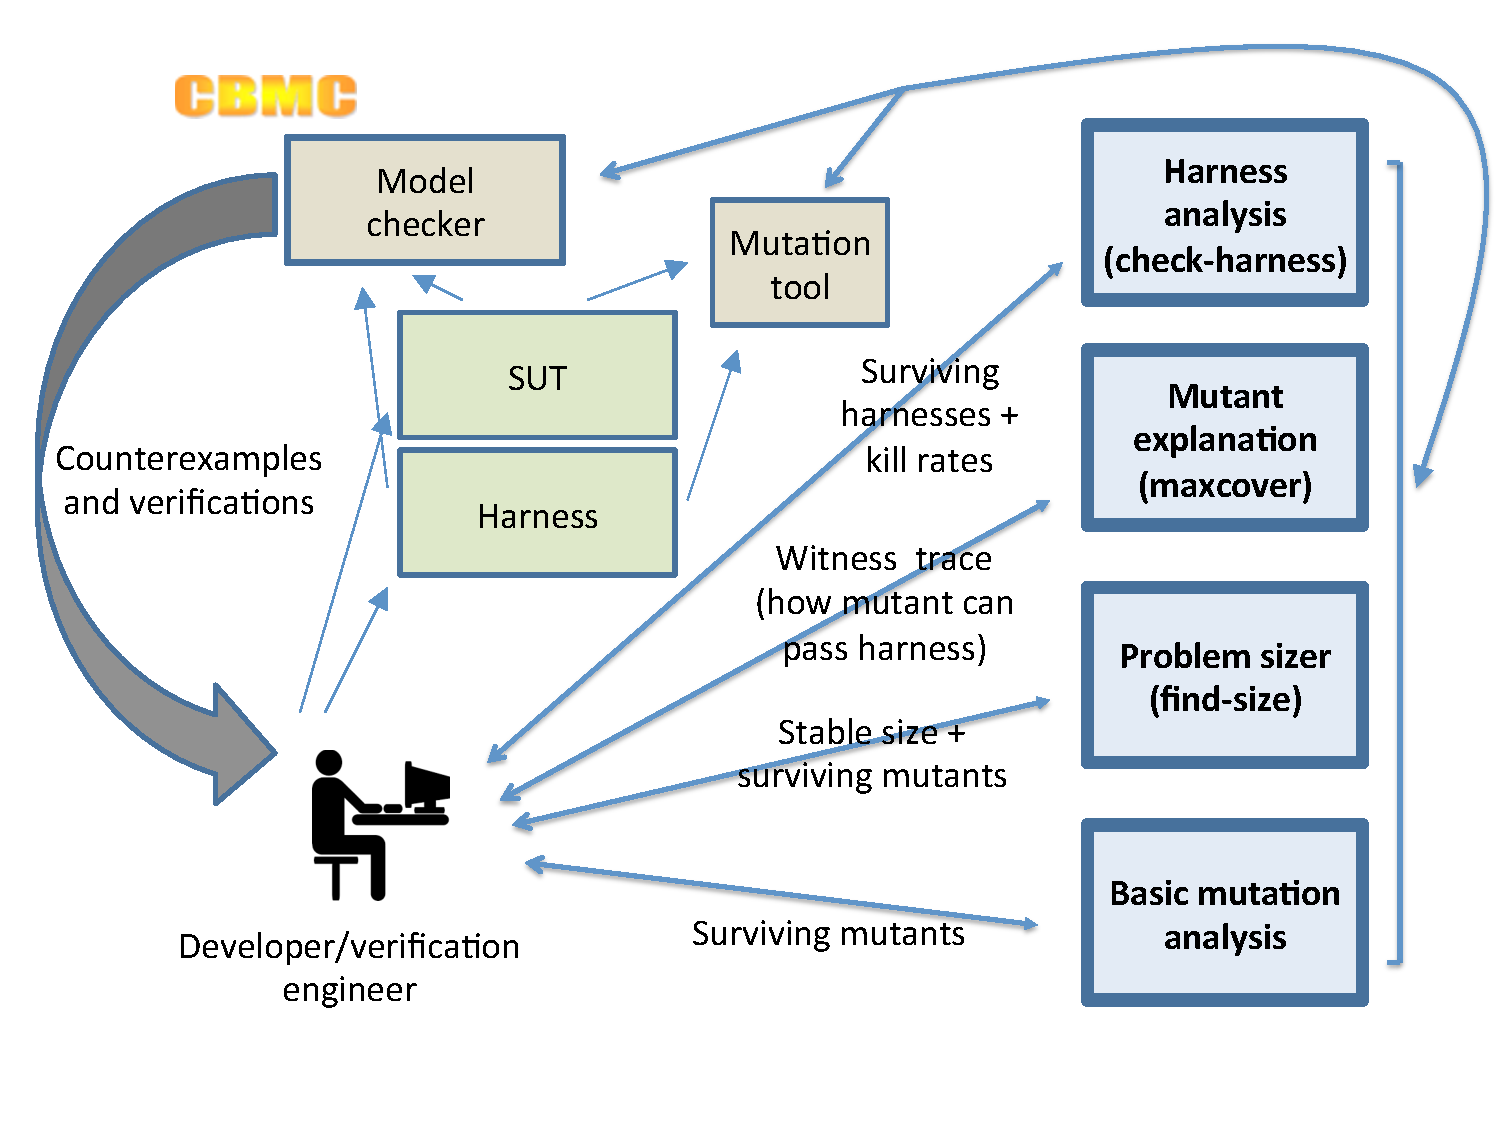
\includegraphics[width=\columnwidth]{TestFlow}
\caption{Basic flow of falsification-driven verification.}
\label{fig:flow}
\end{figure}

\begin{figure}
{%\scriptsize 
\begin{code}
(int, survivors) {\underline{find-size}} ($H$, $M$, $S_0$: int,
                            $O$: int $\rightarrow$ options,
                            $U$: int $\rightarrow$ int) 
\vspace{0.1in}
  S = $S_0$-1 
  r' = \{\} : mutant $\rightarrow$ result
  TOP:
  S = S + 1 
  r = r' 
  r' = \{\}
  for $m \in M$:
     if $m \not\in domain(r)$:
         r[m] = check($H$,$m$,$U(S)$,$O(S)$) 
         if r[m] == VERIFICATION FAILED:
           //once killed, assume always killed 
           $M$ = $M \\ m$
     if r[m] == VERIFICATION SUCCESSFUL:
        r'[m] = check($H$,$m$,$U(S+1)$,$O(S+1)$) 
        if r'[m] == VERIFICATION FAILED:
           $M$ = $M \\ m$
           goto TOP 
  // No result changed, so S is mutant-stable 
  return (S-1, $M$) 
\end{code}
}
\caption{Algorithm 1: Finding size/unwinding bound and surviving
  mutants.}
\label{alg:unwind}
\end{figure}

\begin{figure}
{%\scriptsize 
\begin{code}
harness {\underline{cover-harness}} ($H$, $TARGET$) 
\vspace{0.1in}
  $H'$ = $H$

  for stmt $\in H'$:
     if stmt == assert(P):
        stmt = assume(P);

  cover = [
    assume(total\_coverage >= $TARGET$); 
    assert(!mutant\_covered);]

  insert cover at end of $H'$.main() 

  return $H'$
\end{code}

\vspace{0.2in}

\begin{code}
mutant {\underline{cover-mutant}} ($m$) 
\vspace{0.1in}
  n = 0
  $m'$ = $m$
  for if\_stmt c in $m'$:
     if c has no else:
        add [else \{\}] to c
  for basic\_block b in $m'$:
     b = [if !covered[n] \{
             covered[n] = 1;
             total\_covered += 1;
          \}
          b]
     n = n + 1
  for stmt s in $m'$:
     if MUTANT(s):
        s = [\{mutant\_covered = 1;
              s\}]
  $m'$ = [int total\_covered = 0;
        int mutant\_covered = 0;
        int covered[n];
        $m'$]

  return $m'$
\end{code}

\vspace{0.2in}

\begin{code}
trace {\underline{maxcover}} ($m$, $H$, $S$, $O$, $U$) 
\vspace{0.1in}

  $m'$ = cover-mutant($m$)

  T = 0
  trace = $\emptyset$
  failed = False
  while (not failed)
     $H'$ = cover-harness($H$, T)
     r = scheck($H$,$m'$,$U(S)$,$O(S)$)
     if r == VERIFICATION SUCCESSFUL:
       failed = True
     else if r == VERIFICATION FAILED:
       trace = r.trace
       T = trace.read(total\_covered) + 1
  return trace
\end{code}
}
\caption{Algorithm 2: Find a maximally covering execution trace that
  covers a mutant.}
\label{alg:maxcover}
\end{figure}

\begin{figure}
{%\scriptsize 
\begin{code}
report {\underline{check-harness}} ($SUT$, $M$, $H$, $M(H)$, $S$, $O$, $U$) 
\vspace{0.1in}

  K$_H$ = killed($M$, $H$, $S$) 

  Hkills = $\emptyset$; Hequal = $\emptyset$; Hbetter = $\emptyset$; N = $\emptyset$

  for H$_i$ in $M(H)$:
     original = check($H_i$, $SUT$, $U(S)$, $O(S)$)
     if original == VERIFICATION FAILED: 
        Hkills += H$_i$
     else: // check if this kills fewer mutants
        K$_{H_i}$ = killed($M$, $H$, $S$)
        for k $\in$ K$_{H_i}$:
           if k $\not\in$ K$_H$: N += ($H_i$, k)
        if |K$_{H_i}$| > |K$_H$|:
           Hbetter += (H$_i$, K$_{H_i}$)
        if |K$_{H_i}$| == |K$_H$|:
           Hequal += (H$_i$, K$_{H_i}$)
        else:
           Hkills += (H$_i$, K$_{H_i}$)
  return (Hkills, Hequal, Hbetter, N)
\end{code}
}
\caption{Algorithm 3: Analyze a harness.}
\label{alg:checkharness}
\end{figure}


\subsection{Adapting Falsification-Based Approaches to Automated Test
  Generation}

\subsubsection{Mutants and Manual vs. Automatically Generated Tests}

In this paper, we do not propose the idea of using mutants to improve
manually constructed test cases; that concept is essentially as old as
the idea of mutation testing itself.  Instead we focus on the testing
equivalent of a verification harness: an automated test generation
harness and the tests it produces.  We believe that, despite
superficial similarity, the two ideas are fundamentally different.  In
the first case, there is static, concrete, existing test suite.
Mutation analysis is performed on this suite, and a developer writes
concrete, specific, tests to kill mutants that are not equivalent.
This may be a useful exercise, and may indeed somewhat improve the
future defect detection powers of the suite
\cite{justmutants,ahmed_testedness} to some extent.  We suspect,
however, that this method seldom immediately results in detection of
an existing fault in the SUT.  The developer of the test to kill the
mutant is not, really, looking for a new way to test the system, but
looking for a specific input that causes the mutant to behave
incorrectly.  Again, this may improve the suite, but seems unlikely to
detect other, lurking, incorrect behaviors.  To our knowledge, there
are no human studies showing that such changes result in immediate
fault detection.

However, the story is quite different with an automated test
generation system based on a harness defining tests to be generated,
for instance a sophisticated random test generator for a specific
domain \cite{ICSEDiff,csmith,tstlsttt,rcutorture}.  In that setting,
modifying the harness so that a test is generated that kills the
mutant does more than kill a specific mutant:  it, as in model
checking, extends the generative range of the testing itself, and
(likely) requires a more abstract approach to each mutant than is
possible with specific, manually written tests.  In short, modifying a
test harness that generates an essentially unbounded number of
different tests is not, at a high level, very different than modifying
a verification harness to detect a mutant.  Both operations require
not just an analysis of a specific faulty behavior, but an improvement
to the \emph{testing process}.  The only major difference is that with
test generation, the goal is to achieve high probability of detection,
since the certainty of verification is lost.  In compensation,
however, one receives scalability, ease-of-use, and availability in
languages without formal verification tools.

Note that we propose mutation testing as a way to \emph{extend} the insight
into a test generation effort provided by code coverage \cite{CovDisc}.  When the
generator never produces tests covering a line of code, this can be
detected without the expense or difficulty of producing mutants, and
interpretation is straightforward:  if you are interested in testing
the un-covered code, you must modify the generator to cover it.
Coverage is good at predicting overall mutation scores \cite{ISSTA13,ICSE14},
but there is a gap between coverage's information and that provided by
some surviving mutants.  This gap is our interest.
Mutants provide insight on the strength of the oracle
used to assess generated tests, and the degree to which generated
inputs stress it (a line of code can be covered but not thoroughly
stressed, since coverage does not consider subtle aspects of, e.g.,
expression evaluation).

\subsubsection{Falsification-Driven Testing}

This section explains the
adaptations required to apply our approach in the context of automated
test generation, rather than formal verification.
One aspect of the approach outlined above requires no modifications:
examining mutants that are not killed is the same basic process,
whether those mutants are not killed by a verification harness or a
test generation harness.  Similarly, mutating a test harness is not essentially
different, though it is less useful in testing than in verification
(because of the probabilistic nature of most aggressive testing).  Two
aspects, however, require some modification.

First, and simplest, the method for generating passing executions is
slightly different.  Rather than simply negating the specification and
adding constraints for code coverage, we modify the testing tool (in
our case the TSTL tool for Python \cite{tstlsttt,NFM15} by adding
options to 1) search for a passing test with maximum code coverage and
2) constrain the search to only tests that cover a given statement or
branch.  These options are:  {\tt --trackMaxCoverage <file>}, {\tt
  --maxMustHitBranch <branch>} and {\tt --maxMustHitStatement <stmt>}.

With this addition to TSTL, finding passing executions to examine is
trivial, simply a matter of identifying the location of the mutant.
Adding a similar feature to most widely used test generation tools
should be relatively easy, given that they work by first generating a test, then
executing it and determining its coverage and other properties, such as
whether it passes (or generating a test on the fly while determining
these properties).  

The second change is that the notion of mutant stability changes in
two ways.  First, the parameter to be optimized is different:  while
test generation usually requires a maximum test length \cite{ASE08},
that parameter is not one with a corresponding computational cost,
like a bounded model checking depth.  The same test budget can support
multiple lengths, and there is no simple correspondence between depth
and mutants killed.  Mutants killed is monotonic (stable or
increasing) in bounded model checking depth; mutants killed is not
monotonic in maximum test length \cite{ASE08}.  However, there is an
analogous parameter in test generation:  actual test budget.  This
parameter, however, only produces \emph{probabilistically} \cite{arcuri2014hitchhiker} monotonic
behavior:  one run with budget $X > Y$ may kill fewer mutants than a
run with budget $Y$; however, over a large number of runs,
statistically, $X$-budget tests must outperform, or perform the same
as, $Y$-budget tests.

A key insight is that when estimating how hard a mutant is, a single
run that either takes a long time to kill the mutant or a run that
fails to kill a (known-killable) mutant is sufficient evidence to
assume the mutant is difficult, and helps establish a lower bound on
test budget needed to reduce risk of missing faults; in contrast, a
single run that quickly kills a mutant does not establish that the
mutant is in fact easy:  even hard mutants can sometimes be easy to
detect.  In part we base this idea on empirical evidence (see below),
but it can also be justified by a simple theoretical model of test
generation.  

Unfortunately, the change to a stochastic setting makes determining
stability more difficult.  It is highly inefficient, once budgets
become larger (which is often required in testing), to run each mutant
enough times to obtain a good estimate of how long it takes to kill,
and doing so requires running already killed mutants, or equivalent
mutants, many times.  On the other hand, in another sense the problem
becomes easier:  with bounded model checking, for each mutant $m$, we have
to query wither unwinding depth $U$ is sufficient to kill the mutant,
for each $U$ until stability is achieved.  Many test generation
systems, such as TSTL, support a mode where the tool simply runs until
a fault is detected.  If we set a large timeout (larger than the
largest test budget we are interested in), we can simply run the tool
with each mutant and discover how long it takes to kill it (or if it
cannot be killed within our maximum possible budget).  Finding
``stability'' then, becomes simply a matter of finding the mutant(s)
with the largest time-to-kill, and inspecting those never killed to
determine if they are equivalent.

Unfortunately, again due to the stochastic setting, this is not quite
sufficient.  A hard-to-kill mutant may, by chance, infrequently be
detected very quickly; an easy-to-kill mutant may, by chance,
sometimes not be detected quickly.  Both cases result in inaccurate
information, and potentially in a wrong estimate of the correct test
budget to use.  Fortunately, an asymmetry in the probabilities of
these misleading results allows us to proceed without (usually) running each
mutant many times.

\subsubsection{Estimating Required Budget to Kill a Mutant}


\begin{figure}
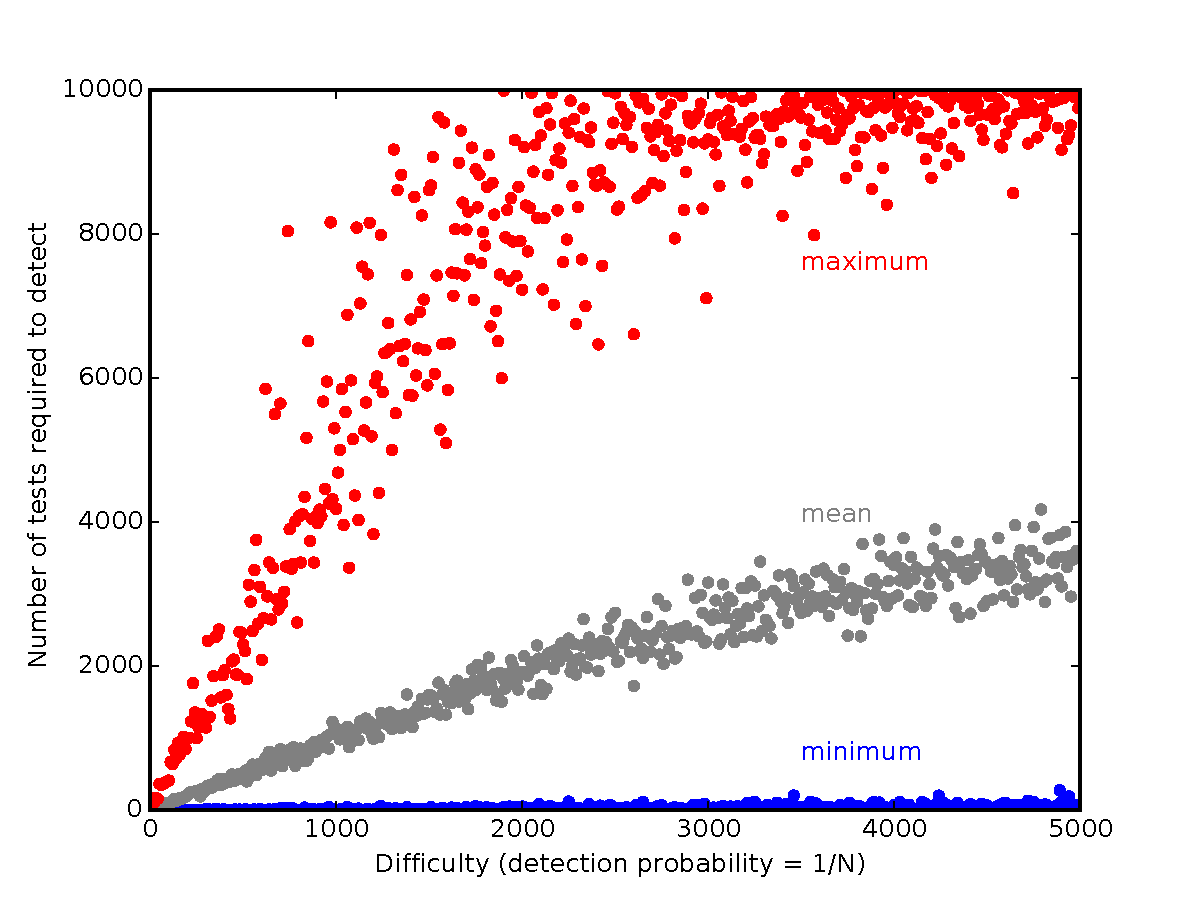
\includegraphics[width=\columnwidth]{probsmodel}
\caption{Tests required for detection as difficult of fault/mutant increases.}
\label{fig:probmodel}
\end{figure}


\begin{figure}
{%\scriptsize 
\begin{code}
float {\underline{stable-budget}} ($M$, $k$, $T$, $maxTime$, $equiv$,$killTimes$)
\vspace{0.1in}
  budget = 0

  for m $\in M$:
     killTime = -1
     runs = 0
     maxKillTime = -1
     while (killTime < budget) and (runs < $k$):
         runs = runs + 1
         // Assume killTime is -1 if not killed
         killTime = $T$(timeout=$maxTime$)
         if killTime > maxKillTime:
            maxKillTime = killTime

     if maxKillTime == -1:
        $equiv$ = $equiv \cup m$
     else:
        $killTimes$[$m$] = maxKillTime

     if maxKillTime > budget:
        budget = killTime
  
  return budget
\end{code}
}
\caption{Estimating needed budget for mutant-stable testing}
\label{alg:testdepth}
\end{figure}

The difficulty of detecting a fault (or killing a mutant, which is
equivalent) can be simply expressed by a probability of detection,
e.g. a trivial fault is detected with almost every generated test
(99/100 tests), a typical easy fault is detected frequently (1/100
tests), and a hard fault is detected two orders of magnitude or more
less frequently (1/5000 tests).  In fact, real faults often seem to
fall into such coarse ``buckets'' of detection ease, though this is not
required for our analysis \cite{PLDI13}.  

Figure \ref{fig:probmodel} shows how the minimum number of tests, mean
number of tests, and maximum number of tests needed for detection,
over 100 runs each consisting of 10,000 tests, vary as the difficulty
of a mutant or fault changes.  For simplicity, we measure difficulty
by increasing $N$, where the probability of detection is $1/N$.  As
you can see, while the maximum number of tests required increases
rapidly, and the mean number of tests also increases steadily, but
much more slowly, with
difficulty, the minimum number of tests required increases very
slowly.  A concrete example shows why: the chance of getting ``lucky'' and hitting a test with
difficulty $1000$ on the first test is indeed small, only $1/1000$.  However, the
chance of getting ``unlucky'' and failing to detect a test with
difficulty $1/10$ for even as few as 100 tests is less than $1/30,000$.


This asymmetry means that as soon as a mutant has taken a long time to kill, we
can safely assume that it is indeed hard to kill; when a mutant is killed
quickly, we run again, based on a tolerance for error in budget
estimation (where each run adds large confidence); after $k$ runs we
assume a mutant is indeed easy (and the chance that we are
over-approximating its ease can be readily computed given $k$, by
standard statistical techniques).  As soon as one
detection takes a long time  we can use that
value as an estimate for the difficulty of the mutant, which means
that we only use $k$ runs if the first $k-1$ runs are all relatively short.  While this
approach is not perfect, it has the huge advantage of never requiring
more than a total runtime slightly more than 1 run with the full test
budget, unless $k$ is large.  Of course, there is the question:  what
is a ``long time'' to kill a mutant?  If our goal is to set a test
budget, the answer is that a mutant takes a long time to kill if it
takes longer than any previously killed mutant (where mutants that
have not been killed at all do not increase this threshold).  This
means that the expensive mutants (requiring $k$ long runs) are those
that (1) cannot be killed, or are at least highly unlikely to be
killed or (2) require time close to the current estimated
budget, but not exceeding it.  If the goal is simply to classify
mutants as ``easy'' or ``hard'' based on some threshold, however, the
``bad cases'' can be made much less frequent.

More precisely, to coarsely, but
cheaply, estimate a stable test
budget for a set of mutants, we use the procedure in Figure
\ref{alg:testdepth}, which returns a budget and modifies a set of
possibly equivalent mutants.  The procedure is also designed to store a
difficulty for each mutant, in addition to an overall budget, by simply storing the largest {\tt
  killTime} for that mutant.  The procedure takes as input a set of
mutants $M$, a number of trials $k$, a test procedure $T$, a maximum
test budget to use, $maxTime$, a (modifiable) structure to store
possibly equivalent mutants, $equiv$, and a similar structure (except
a map), $killTimes$ to store the maximum kill times for each mutant.
It is this map that allows us to use standard statistical techniques
to derive budget tradeoffs.  Given this (admittedly very approximate, since the
procedure is intended to set a budget, not evaluate each mutant) distribution of expected actual
kill times based on the reported maximum kill times, it is also easy to
solve for (or use Monte Carlo methods to estimate) budgets that kill
any given percent of mutants, or all killable mutants, with a certain
required confidence.

\section{Case Studies and Experimental Results}

\subsection{Algorithm Implementations}

Our initial experiments involved relatively small verification
problems, based on implementations taken from the web or student code for popular
algorithms and data structures.  Here we highlight the most
interesting of these; we also successfully applied the method to
bubble sort and a student's harness for verifying a version of Dijkstra's
shortest path algorithm that enables path reconstruction \cite{dijkstrasp}.  For the Dijkstra
harness, the low mutant kill rate of only 58\% showed that while the
harness checks incorrect returned paths, it cannot detect when return
values indicate there is no path but one exists.  Improving the
harness is a substantial exercise, but can be guided by the survival witnesses.

\subsubsection{Binary Search}

The ideas in this paper grew out of a side project of the first
author: to write a follow-up to Jon Bentley's article on verifying
binary search \cite{Bentley} in the context of modern software
verification tools (and Joshua Bloch's discovery of a bug in the
assumptions behind Bentley's proof \cite{Bloch}).  The modeling
required is moderately complex (to scale well, an abstract ``sorted
array'' that represents all sorted arrays but only introduces
variables equal to the number of probes made by the search is
essential).  In this case, we did not produce an initial, weaker
version of the harness, but checked the existing harness using
mutants, and determined that all 3 surviving mutants are equivalent to
a true binary search.

Checking harness mutants (which took 37 minutes, including computing
the kills for the original harness) produced results confirming the belief this is a
good harness.  Of the 31 compiling harness mutants, 19 failed to verify
the correct binary search, and 7 had worse kill rates than the
original harness.  The remaining 5 harnesses, all with equal kill
rates of 86.7\%, all modify an assumption to allow the harness to also
check size 0 arrays.  This doesn't kill any additional mutants, but is
harmless as expected.  Of the harness mutants with worse kill rates,
three are mutants of the assumptions on the nondeterministic value used to
make sure that if binary search returns -1, no index in the array
actually contains the searched-for item.  Two of these mutants are
off-by-one-errors that exclude item 0 from the check, an easy-to-make
mistake.  Both of these fail to kill \emph{exactly} one mutant killed by the
correct harness: the mutant that sets the lower bound
initially to 1 instead of 0.  Traces of passing runs for these mutants show the
problem clearly (the sought item at index 0).

\subsubsection{Doubly-linked-list Insertion Sort}

Another example, making use of recursive data structures and pointer
validity checks, is code for inserting an item (in
sorted order) into a doubly-linked list \cite{DLLInsert}.  Our initial
harness omitted a check for correctness of {\tt prev} pointers.  This
problem didn't directly prevent mutants from being detected, but
pushed the stable size larger, as with the quicksort example above.
Looking at a trace of a size 3 run that fails to kill a clearly
problematic mutant easily reveals the problem (the results are correct
up to {\tt prev} pointers).  This example also showed another use of
mutants, in that some seemingly problematic surviving mutants actually
just showed a pointless redundancy in the implementation, enabling the
removal of an entire conditional branch.  A harness check (requiring
30 minutes, including computing the mutant kills for the original
harness) showed that of the 105 compiling harness mutants, 92 fail to
verify the original code.  Another 2 have a worse kill rate than the
original (which kills 81\% of mutants, a low rate due to the code
redundancy), and 11 survive.  The large number of survivors is due to
a redundancy of the final harness, which checks sortedness and the
permutation property for both a forward {\tt next} traversal of the
list and a {\tt prev} traversal.  Omitting any \emph{one} of these
(e.g. {\tt prev} sortedness or {\tt next} permutation) the harness can
still detect all mutants.  Removing two, however, fails to kill
mutants.  The two harness mutants with worse kill rates have extremely poor
kill rates ($<50$\% and $<25$\%).

\subsubsection{AVL Tree}

In the case of the AVL tree, the harness we were working with
was unable to reach a mutant-stable unwinding without exhausting
memory on the verification of the main program (for AVL trees of up to
size 5).  We are investigating a more efficient harness encoding,
based on the inability to reach mutant-stability.  Without the notion
of mutant-stability, we might have believed the harness was verifying
more aspects of the specification than it is able to, at the largest
unwinding reached.  Unkilled mutants include clearly erroneous behaviors.


\subsubsection{Merge With Duplicate Removal}
\begin{figure}
{%\scriptsize
\begin{code}
int main () \{
  int a[SIZE], b[SIZE], c[SIZE*2];
  int i, v, i1, i2, csize;
  int asize = nondet\_int();
  int bsize = nondet\_int();
  \_\_CPROVER\_assume ((asize >= 0) \&\& (bsize >=0));
  \_\_CPROVER\_assume ((asize <= SIZE) \&\& (bsize <= SIZE));
  for (i = 0; i < asize; i++) \{
    a[i] = nondet\_int();
    \_\_CPROVER\_assume((i == 0) || (a[i] >= a[i-1]));
  \}
  for (i = 0; i < bsize; i++) \{
    b[i] = nondet\_int();
    \_\_CPROVER\_assume((i == 0) || (b[i] >= b[i-1]));
  \}
  csize = merge\_sorted\_nodups(a, asize, b, bsize, c);
  assert (csize <= (asize + bsize));
  i1 = nondet\_int();
  i2 = nondet\_int();
  \_\_CPROVER\_assume((i1 >= 0) \&\& (i2 >= 0));
  \_\_CPROVER\_assume((i1 < csize) \& \& (i2 < csize));
  \_\_CPROVER\_assume(i1 != i2);
  assert(c[i1] != c[i2]);
  v = nondet\_int();
  \_\_CPROVER\_assume ((v >= 0) \&\& (v < asize));
  v = a[v];
  int found = 0;
  for (i = 0; i < csize; i++) \{
    if (c[i] == v)
      found = 1;
  \}
  assert (found == 1);
  v = nondet\_int();
  \_\_CPROVER\_assume ((v >= 0) \&\& (v < bsize));
  v = b[v];
  int found = 0;
  for (i = 0; i < csize; i++) \{
    if (c[i] == v)
      found = 1;
  \}
  assert (found == 1);
\}
\end{code}
}
\caption{Harness for merge\_sorted\_nodups}
\label{fig:mergeharness}
\end{figure}

\begin{figure}
{%\scriptsize
\begin{code}
int merge\_sorted\_nodups(int a[], int asize, 
                        int b[], int bsize, int c[]) \{
  int apos = 0, bpos = 0, cpos = -1, csize = 0;
  while ((apos < asize) || (bpos < bsize)) \{
    if ((apos < asize) \&\& 
        ((bpos >= bsize) || (a[apos] < b[bpos]))) \{
      if ((cpos == -1) || (c[cpos] != a[apos])) \{
	c[++cpos] = a[apos];
	csize++;
      \}
      apos++;
    \} else \{
      if ((cpos == -1) || (c[cpos] != b[bpos])) \{
	c[++cpos] = b[bpos];
	csize++;
      \}
      bpos++;      
    \}
  \}
  return csize;
\}
\end{code}
}
\caption{Code to merge two sorted arrays into one sorted array with no
  duplicate elements}
\label{fig:sortnodup}
\end{figure}


Even a killed mutant---one the harness does detect---can shed
critical light on harness vulnerabilities.  For example, the code in
Figure \ref{fig:mergeharness} is a portion of a harness to verify
code that merges two sorted arrays, removing all duplicates (the
source arrays may contain duplicates or shared items, the output array
is guaranteed to be sorted and have all-unique values).  This harness
detects all non-equivalent mutants of the source code with an
unwinding depth of only 2 (the check requires less than a minute).

However, as is
well known, many software faults \cite{justmutants} are not
represented by a mutant.  Because we are model checking, we want our
harness to actually rule out \emph{all} bad runs of the program under
test.  Even a killed mutant's passing executions may show such a
problem.  Here we see that when the output array's size is 1, the way
we have written the duplicate check in fact \emph{assume}s away
\emph{all executions}!  We check no properties of size 1 output
arrays, and a fault that only appears with size = 1 will never be
detected.  No mutant produces such behavior, but noting an incorrect
but passing trace of this run using the CBMC extension lets us see the problem.

\subsection{SpiderMonkey Boyer-Moore-Horspool Implementation}

\begin{figure}
{%\scriptsize
\begin{code}
jsint
js\_BoyerMooreHorspool(const jschar *text, jsint textlen,
                      const jschar *pat, jsint patlen,
                      jsint start)
\{
  jsint i, j, k, m;
  uint8 skip[BMH\_CHARSET\_SIZE];
  jschar c;

  JS\_ASSERT(0 < patlen && patlen <= BMH\_PATLEN\_MAX);
  for (i = 0; i < BMH\_CHARSET\_SIZE; i++)
    skip[i] = (uint8)patlen;
  m = patlen - 1;
  for (i = 0; i < m; i++) \{
    c = pat[i];
    if (c >= BMH\_CHARSET\_SIZE)
      return BMH\_BAD\_PATTERN;
    skip[c] = (uint8)(m - i);
  \}
  for (k = start + m;
       k < textlen;
       k += ((c = text[k]) >= BMH\_CHARSET\_SIZE) ? 
             patlen : skip[c]) \{
    for (i = k, j = m; ; i--, j--) \{
      if (j < 0)
	return i + 1;
      if (text[i] != pat[j])
	break;
    \}
  \}
  return -1;
\}
\end{code}
}
\caption{SpiderMonkey 1.6 Boyer-Moore-Horspool code.}
\label{fig:bmh}
\end{figure}

\begin{figure}
{%\scriptsize
\begin{code}
\#include "bmh.h"
int main() \{
  int i;
  unsigned int v;

  char itext[TSIZE];
  char ipat[PSIZE];

  unsigned int itext\_s = nondet\_uint();
  \_\_CPROVER\_assume(itext\_s < TSIZE);
  unsigned int ipat\_s = nondet\_uint();
  \_\_CPROVER\_assume(ipat\_s < PSIZE);

  printf ("LOG: size text=\%u, pat=\%u\\n", itext\_s, ipat\_s);

  for (i = 0; i < itext\_s; i++) \{
    v = nondet\_unit();
    \_\_CPROVER\_assume((long)v < (long)BMH\_CHARSET\_SIZE);
    itext[i] = v;
    \_\_CPROVER\_assume(itext[i] < BMH\_CHARSET\_SIZE);
    printf ("LOG: text[\%d] = \%u\\n", i, itext[i]);
  \}

  for (i = 0; i < ipat\_s; i++) \{
    v = nondet\_uint();
    \_\_CPROVER\_assume((long)v < (long)BMH\_CHARSET\_SIZE);
    ipat[i] = v;
    \_\_CPROVER\_assume(ipat[i] < BMH\_CHARSET\_SIZE);
    printf ("LOG: pat[\%d] = \%u\\n", i, ipat[i]);
  \}

  jsint r = js\_BoyerMooreHorspool(itext, itext\_s, 
                ipat, ipat\_s, 0);

  printf ("LOG: return = \%d\\n", r);
  
  int pos, ppos, found;

  v = nondet\_uint();
  printf ("LOG: looking at \%u\\n", v);
  \_\_CPROVER\_assume(v >= 0);
  
  if (r == -1) \{
    \_\_CPROVER\_assume(v < itext\_s);
    pos = v; ppos = 0; found = 1;
    while (ppos < ipat\_s) \{
      printf ("LOG: itext[\%d] = \%u, ipat[\%d] = \%u\\n",
                 pos, itext[pos], ppos, ipat[ppos]);      
      if ((pos>=itext\_s)||(itext[pos]!=ipat[ppos])) \{
	found = 0; break;
      \}
      pos++; ppos++;
    \}
    assert (!found);
  \} else \{
    pos = r; ppos = 0;
    while (ppos < ipat\_s) \{
      assert (itext[pos] == ipat[ppos]);
      pos++; ppos++;
    \}
    v = nondet\_uint();
    printf ("LOG: looking at \%u\\n", v);
    \_\_CPROVER\_assume(v < r);
    pos = v; ppos = 0; found = 1;
    while (ppos < ipat\_s) \{
      printf ("LOG: itext[\%d] = \%u, ipat[\%d] = \%u\\n",
                 pos, itext[pos], ppos, ipat[ppos]);
      if ((pos>=itext\_s)||(itext[pos]!=ipat[ppos])) \{
	found = 0; break;
      \}
      pos++; ppos++;
    \}
    assert (!found);
  \}
\}
\end{code}
}
\caption{Boyer-Moore-Horspool harness.}
\label{fig:bmhharn}
\end{figure}

Figures \ref{fig:bmh} and \ref{fig:bmhharn} show, respectively, the
source code and an initial harness for verification of the
Boyer-Moore-Horspool substring finding algorithm \cite{BMH,CFV13} in
version 1.6 of Mozilla's SpiderMonkey JavaScript engine.  Verifying
this code presents one immediate issue that is not unusual in
verification: how to handle an {\tt assert} in the code being
verified.  An {\tt assert} at the end of a function or in the main
body is typically an additional part of the specification, and is
often best left unchanged.  An {\tt assert} at the beginning of a
function's body, however, is typically a precondition for the code \cite{CFV13}.  It is natural to consider changing such an assertion into
an {\tt assume} and ignoring any problems produced by calling the code
with non-conforming inputs.  While this can be a useful technique (for
instance when it is hard to write a harness that only produces valid
inputs, but easy to filter out the invalid inputs and only verify
behavior for those) it is also a dangerous technique.  Mutation
analysis of the harness shows that 4 is a mutant-stable size (where
the same size is used for text length, pattern length, and character
set size), with a kill rate of 72.3\%.  On initial examination, the 20
surviving mutants do not seem problematic.  A large number involve the
{\tt JS\_ASSERT} converted to a {\tt \_\_CPROVER\_assume}, showing the
harness cannot tell if the assumption is incorrect, which is not
surprising (the harness only generates good inputs, and some of the
mutants simply discard too many inputs).

At this point, we were satisfied with our harness, and ran a check on
mutants of the harness itself.  To our surprise, three mutants of the
harness had a better kill rate than the ``correct'' harness, killing
73.5\% of mutants.  Investigating these ``better'' harnesses showed
mutants that broke processing of some return values in such a way
that, while these harnesses failed to detect certain major bugs in the
code, they were able to detect some {\tt JS\_ASSERT} assumption
mutants.  Guided by this, we produced a revised harness that raised
the kill rate to 79.52\%.  However, on examining the surviving
mutants, we realized that our verification was still unsatisfactory as
a good regression for the Boyer-Moore-Horspool code: in particular, if
the assertion were ever modified to allow bad inputs to pass through,
or otherwise incorrectly changed, we would those bugs.  We then
changed the {\tt JS\_ASSERT} into code that returned a special value
to signal assertion failure, and modified the harness once more,
allowing some incorrect values to pass through and checking that
``assertion failure'' happened if, and only if, the inputs were
invalid.  This harness killed 89.2\% of mutants, and the six surviving
mutants were easily understood to be equivalent to the BMH code under
all valid inputs (in one case we weren't certain about, we had CBMC
verify that for all non-assertion violating inputs, this was true up
to size 10).  The new harness, informed by the harness mutations, in
fact had a better mutant kill rate for size 3 (80.7\%) than our first
harness had at the mutant-stable point.  This examples serves as our
best evidence of the value of harness mutation.

\subsection{Linux Kernel RCU Verification Challenges}

%\subsubsection{Introduction to RCU}


Read-Copy-Update (RCU) is a synchronization mechanism sometimes used as a replacement
for reader-writer locking for linked structures, allowing extremely
lightweight readers \cite{McKenney:2013:SDS:2483852.2483867}.
In the limiting case, achieved in server-class builds of the
Linux kernel, overhead for entering and exiting an \emph{RCU read-side
critical section} (using {\tt rcu\_read\_lock()} and {\tt rcu\_read\_unlock()},
respectively) is exactly zero \cite{McKenney98}, making RCU an
excellent choice for read-mostly workloads
\cite{McKenney:2013:SDS:2483852.2483867,DinakarGuniguntala2008IBMSysJ,PaulMcKenney2013AMPenergyHOTPAR}.  
However, lightweight readers mean updaters cannot exclude readers, so updaters must take care to avoid disrupting readers.
Updaters typically maintain multiple versions of the portion of the
data structure being updated, removing old versions only when
readers are no longer accessing them.
To this end, RCU provides {\tt synchronize\_rcu()}, which waits for a
\emph{grace period}: when all pre-existing RCU readers complete.
RCU updaters typically remove a data element (rendering it
inaccessible to new readers), invoke {\tt synchronize\_rcu()},
and then reclaim a removed element.
\begin{comment}Production-quality implementations of {\tt synchronize\_rcu()} use batching
techniques to achieve extremely scalability, so that a single underlying
grace period can satisfy more than 1,000 concurrent updates in the
Linux kernel~\cite{Sarma04c}.\end{comment}
The Linux kernel contains more than 10,000 uses of the RCU
API \cite{PaulEMcKenneyRCUusagePage}, and a userspace RCU
library \cite{MathieuDesnoyers2009URCU,MathieuDesnoyers2012URCU}
is seeing significant use.  Validation and verification of RCU is a
major concern for each implementation, and a topic of considerable
interest in the PL/verification community now \cite{PLDI15RCU}.

\begin{comment}
\emph{Should we cite this? 
\url{http://conf.researchr.org/event/pldi2015/pldi2015-papers-verifying-read-copy-update-in-a-logic-for-weak-memory}}
\end{comment}


\begin{comment}{The {\tt rcutorture} stress-test suite qualifies, but it would be
good to evaluate its effectiveness on the one hand
(via permutation analysis)
and to include formal verification on the other.
However, regression-test use of formal verification required that
the following properties:
(1)~Direct use of source code,
(2)~Automatic discarding of irrelevant source statements,
(3)~Reasonable memory and CPU overhead,
(4)~Automatic mapping of error reports to source lines, and
(5)~Modest additional input beyond the source code.
Failing to provide any of these requirements provides unacceptable
vulnerability to human error.
This raise the question of whether readily available formal-verification
tools meet these requirements.}
\end{comment}

\begin{figure}[tb]
{ %\scriptsize
\begin{verbatim}
 1 static int rcu_read_nesting_global;
 2 
 3 static void rcu_read_lock(void)
 4 {
 5   (void)__sync_fetch_and_add(&rcu_read_nesting_global, 2);
 6 }
 7 
 8 static void rcu_read_unlock(void)
 9 {
10   (void)__sync_fetch_and_add(&rcu_read_nesting_global, -2);
11 }
12 
13 static void synchronize_rcu(void)
14 {
15  for (;;) {
16   if (__sync_fetch_and_xor(&rcu_read_nesting_global, 1)<2)
17     return;
18   SET_NOASSERT();
19   return;
20  }
21 }
\end{verbatim}
}
\caption{Approximate model of RCU}
\label{fig:Approximate Model of RCU}
\end{figure}

Because both RCU and the Linux kernel are moving targets, any validation
and verification must be both automated and repeatable, for inclusion
in a regression-test suite.  At present the {\tt rcutorture}
stress-test \cite{rcutorture} provides some assurance in the form of automated testing,
but ideally would be complemented by some formal verification of the
implementation(s) in the kernel.  An important question is whether
available formal verification tools can provide effective additional
regression checking for RCU.
We use a pair of RCU-related benchmarks \cite{PaulBlog1,PaulBlog2} to
provide the beginnings of an answer to this question.  The first
benchmark applies formal verification to the simplest of the Linux
kernel's RCU implementations, Tiny RCU
\cite{PaulEMcKenney2009BloatwatchRCU}, which targets single-CPU
systems.  This model includes Tiny RCU's handling of idle CPUs as well
as its (trivial) grace-period detection scheme.  The second benchmark
creates the trivial model approximating an RCU implementation for
multiprocessor systems shown in Figure \ref{fig:Approximate Model of
  RCU}.  In this model, the number of RCU read-side critical sections
currently in flight is tracked by the global
{\tt rcu\_read\_nesting\_global}, which is atomically incremented by
{\tt rcu\_read\_lock()} and atomically decremented by
{\tt rcu\_read\_unlock()}.  This allows {\tt synchronize\_rcu()} to
atomically XOR {\tt rcu\_read\_nesting\_global}'s bottom bit to detect
whether the current execution has waited for all pre-existing readers
(over-approximated by checking the absence of all readers), with
{\tt SET\_NOASSERT()} being invoked to suppress all future assertions.
Although this model has a number of shortcomings, perhaps most
prominently excessive read-side ordering, it is capable of detecting
common RCU-usage bugs, including failure to wait for an RCU grace
period and failure to enclose read-side references in an RCU read-side
critical section.  Can falsification aid in these two complex,
in-progress, verification efforts?

Our efforts are ongoing, due to the complexity of the targeted code
(even with support from the primary developer, a co-author of this
paper).  At this time the investigation of mutants has already
provided valuable information about these verifications benchmarks.
First, there are two versions of the Tiny RCU verification.  The
earliest, very preliminary version, kills only 10 of 169 Tiny RCU
mutants.  Adding code to the harness to account for interrupts in the
dyntick-idle handling kills an additional 12 mutants, confirming that
the modification increases the strength of the harness.  More
importantly, the modeling of concurrency in the harness has two
versions, one using CBMC support for pthread mutex locks, the other
using disabling of assertions to ignore executions that violate
locking semantics.  The native mutex version allows much faster
verification, and catches the original, hand-constructed checks to
ensure the harness can detect faults in Tiny RCU.  However, the native
mutex version fails to kill any mutants, a fact we are currently
investigating: without mutants, we would not have been aware of this
possibly critical problem, which may be a CBMC bug (in the course of
this paper's work, we have uncovered several CBMC bugs) or a harness
flaw.  In support of the verification, we also generated passing
maximal-coverage executions for all mutants of the Tiny RCU code.  For
97 of the mutants, there is no passing execution; in many cases, these
are not killed: the mutant modifies the concurrency semantics so CBMC
has no valid executions to analyze (potentially invalid in some cases,
which must be investigated).  For 79 mutants the maximal-coverage
passing runs are currently being examined, to determine the best next
steps in improving the Tiny RCU harness.  For the second benchmark, we
have computed mutant kills and find that the kill rates range between
40\% and 46\%.  While these benchmarks are far from complete, and
over-simplify the modeling process, they are already able to catch a
substantial number of potential RCU usage errors.  Again, we have
produced passing runs for the surviving mutants to use in enhancing
the process.  The good news is that while the RCU verification is much
more substantial than the above case studies, the time to analyze
mutants is not prohibitive.  No single model checking run for the Tiny
RCU benchmark takes more than 40 seconds, and total runtime for all
mutants in the usage benchmarks ranges from just over 12 seconds for a
basic litmus test to less than 5 minutes for the most complex of the
benchmarks. \begin{comment} Our belief that analyzing all surviving mutants is
plausible for code of this size and criticality is supported by our
concurrent preliminary work on using mutants to analyze the
effectiveness of {\tt rcutorture}, which has improved {\tt rcutorture}
itself and (by doing so) exposed previously undetected RCU bugs.|

Nevertheless, it is important to note that these two benchmarks are not
examples of useful verifications, but rather the simplest examples of
a class that might some day expand to include useful verifications.

(And of course, CBMC proved capable of handling simple variable-pair
litmus tests, as well as single-threaded examples involving linked lists,
but proved incapable of handling multi-threaded tests involving linked
lists.
The maintainers of CBMC are working to improve its handling of pointers.)
\end{comment}

\subsection{Plausible Verification by Failure to Falsify}
\label{sec:sattimes}

\begin{figure}
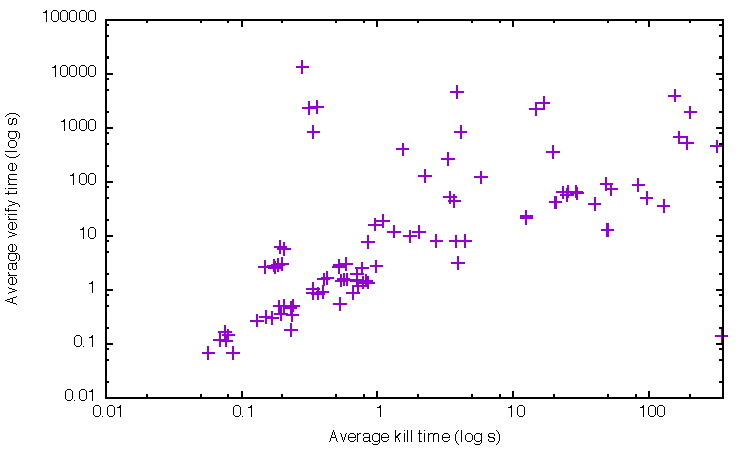
\includegraphics[width=\columnwidth]{sattimes}
\caption{Average times for killing/verifying mutants, in seconds.}
\label{fig:sattimes}
\end{figure}

A key problem in model checking is the state explosion problem, or,
more simply (and more accurately, in that number of states is not
always the determining factor in symbolic methods) the problem of
scalability.  As discussed above, even proving binary search correct
over the full domain of integer inputs is not possible within a
reasonable time frame.  Even when verification is impossible at the
desired problem size falsification can provide limited
confidence in the correctness of a program.  In particular, we observe
from all of our experiments that the average time, for any program and
harness pair, to verify the original code and all surviving mutants is
much higher than the average time to produce a counterexample
for killed mutants.  Showing that a constraint is satisfiable is,
usually, easier than proving it is unsatisfiable.  This is not limited
to SAT solvers; we used SAT rather than SMT in our experiments because
we generally found Z3 to be slower than CBMC's built in version of
MiniSAT\cite{minisat} in almost all cases, but Z3 also
aims to be fast at producing satisfying assignments, not proving UNSAT
\cite{z3}, and our few runs with Z3 showed the same pattern.

Figure \ref{fig:sattimes} shows (with log scales on both axes) the
average running times for all experiments (including faulty versions
of the harness, incorrect runtime parameters, harness mutation checks,
etc.) performed in the course of this work.  The general trend is
clear: time to verify is usually worse than time to kill, and the
worst average time to kill (about 350 seconds) is much better than
many average verification times.  One use of this relationship is
that, in cases where all (non-equivalent) mutants of the SUT are
killed, but the SUT verification fails to complete, the SUT might be
considered provisionally verified. In particular, the larger
the ratio between the timeout for failed verification and the longest
kill time for any mutant, the ``more likely'' to be correct we can
consider the SUT (the same holds with respect to memory use
limits). This belief can be further justified by modifying the harness
to force mutant kills to use large problem sizes, violating the usual
inclusiveness rule (that way, if the new size allows a counterexample
not previously existing, the mutant killing problem for mutants
killable at smaller sizes better approximates the counterexample
construction problem for the actual fault).

Additionally, the times shown here (with mean mutant kill time of 16.4
seconds and median mutant kill time of 0.54 seconds) show the general
feasibility of the falsification-driven approach.  Most of the time,
killing mutants is cost-effective.  The outliers come from a few
difficult problems, arising from buggy harnesses (or harness mutants
that resemble buggy harnesses).  The much worse cost for surviving
mutants is due to a few expensive stubborn mutants: the median
verification success time is only 1.5 seconds.

\subsection{Automated Test Generation and Falsification}

\subsubsection {{\tt rcutorture} Case Study}

In a first effort to integrate our approach with automated test generation, we applied our method to {\tt rcutorture} \cite{rcutorture}
itself \cite{mutKernel}.  While the model checking harnesses we were working with were
weak and limited, {\tt rcutorture} is the workhorse of RCU testing,
and has resulted in detection of numerous bugs.  We generated, again
using Andrews' tool, 2,815 valid (compilable) mutants (and 354 invalid
mutants).  After throwing out
all mutants that were equivalent or
redundant via TCE \cite{TCE}, we ran {\tt rcutorture} for two minutes
on each of the 2,150
remaining mutants.  Two minutes is actual testing
budget; each mutant took up to 30 minutes to compile in the first
place (build failures usually took less time), and a
1-time setup cost of about 30 minutes to produce an image for use in
future testing, if we wanted to run {\tt rcutorture} for longer runs
(this time without compilation or image-production overhead).
Of these 2,150 mutants, only 380 survived the process, yielding an
82\% kill rate, showing
that {\tt rcutorture} is indeed quite effective at detecting most
deviations from the code, and that the code is relatively tightly
constrained in behavior.

Manual inspection by the RCU developer (author McKenney) required
about 5 minutes per mutant, but with very high variance.  Some mutants were
immediately dismissed as irrelevant, while other required considerable
effort.  A good estimate for overall human effort in this case is 25
hours.  This is a significant investment of time, but the payoff, in
this case, was substantial.  In general, the mutants that resulted in
changes to kernel code were also mutants that required substantial
analysis time.

The results of mutation analysis were five patches to RCU code.  Two
of these patches were to {\tt rcutorture} code, improving the testing
process.  Three were patches to RCU code, including one actual bug
fix for a bug detected by the changes to {\tt rcutorture}.  Another
change to RCU was a performance improvement, avoiding the overhead of
a {\tt local\_irq\_save()}/{\tt local\_irq\_restore} pair, since
surviving mutants showed that interrupts were always disabled.  A
final patch more precisely specified a type, again based on
information from mutation testing.  Patch details are available at:

\begin{itemize}
\item \url{https://git.kernel.org/pub/scm/linux/kernel/git/tip/tip.git/commit/?id=45fed3e7cfb4001c80cd4bd25249d194a52bfed3}
\item \url{https://git.kernel.org/pub/scm/linux/kernel/git/tip/tip.git/commit/?id=7c9906ca5e582a773fff696975e312cef58a7386}
\item \url{https://git.kernel.org/pub/scm/linux/kernel/git/tip/tip.git/commit/?id=ca1d51ed9809a99d71c23a343b3acd3fd4ad8cbe}
\item \url{https://git.kernel.org/pub/scm/linux/kernel/git/tip/tip.git/commit/?id=6e91f8cb138625be96070b778d9ba71ce520ea7e}
\item \url{https://git.kernel.org/pub/scm/linux/kernel/git/tip/tip.git/commit/?id=f13bad9042dcf9b60b48a0137951b614a2ee24b5}
\end{itemize}

More details of our {\tt rcutorture} analysis are available in a
workshop paper presented at the 2017 International Workshop on
Mutation Testing \cite{mutKernel}.

\subsubsection {{\tt pyfakefs} Case Study}

We used the a test harness written in  the TSTL
\cite{NFM15,ISSTA15,tstlsttt,tstl} automated test generation language for
testing {\tt pyfakefs} \cite{pyfakefs} as a second case study in applying our approach
to aggressive testing.  The {\tt pyfakefs} module is a widely-used
tool for Python testing that allows tests to replace real file system
usage with the use of a ``fake file system'' that can contain
arbitrary contents, operate faster than a real file system, avoid
tests modifying the real file system, and allow fault injection.  The
harness for {\tt pyfakefs} is a TSTL-based differential testing
harness conceptually similar to harnesses used at NASA for file system
testing \cite{ICSEDiff,CFV08}.  The TSTL tools support a number of testing
methods, but in this case study we restricted ourselves to pure random testing.

The muupi \cite{muupi} mutation generation tool generated 873
mutants of the file {\tt fake\_filesystem.py}, the tested part of the
{\tt pyfakefs} system.  At the time we generated mutants, testing of
{\tt pyfakefs} had been going on for a period of months, with many
changes and extensions of the test harness, leading to discovery and
correction of more than 50 bugs\footnote{See the issues labeled with
  {\bf TSTL} on the pyfakefs GitHub issue tracker for a history of the
  testing effort.}  Of the 873 mutants, only 449 (51.4\%) were actually covered
within 30 minutes of testing {\tt pyfakefs}, and so we omitted the
mutants of code not covered.  Coverage information itself is useful,
and showed some (known) limitations of the testing, but, as discussed
above, we are interested in the additional information on oracle and
input generation strength provided by mutation testing results.

The harness killed 288 of the 449 covered mutants (64.1\%), all within 60
seconds.  For 279 of these, 5 of 5 attempts to kill within 60 seconds
succeeded.  For another 7, fewer than 5 (but not less than 3) attempts
to kill in 60 seconds succeeded.  Extending the test budget to five
minutes did not add any newly killed mutants.  The mean minimum time
to kill a mutant was 0.59 seconds, and the mean maximum time was 3.25
seconds.  The longest minimum time to kill a mutant was 44.8 seconds,
and the longest mean time to kill a mutant was 42.64 seconds.
Our mutation results suggest that 45 seconds of testing is likely to
be as effective as 60 seconds (or five minutes) of testing for {\tt
  pyfakefs}.

\begin{table}
\caption{Easily ignored unkilled mutant categories}
{%\scriptsize
\begin{tabular}{l|l|r}
Identifier & Explanation & Count \\
\hline
{\tt ChangeDiskUsage} & Disk usage is hard to model in differential
                        testing & 8 \\
{\tt usage\_change} & Disk usage is hard to model in differential
                      testing & 2 \\
{\tt \_last\_dev} & Differential testing only uses one device & 4\\
{\tt \_last\_ino} & inode usage not modeled in differential testing &
                                                                      8\\
{\tt epoch} & epoch not modeled in differential testing & 3\\
{\tt link\_depth} & link depth is limited by assumption in testing & 4\\
{\tt reversed} & reversing lists used as sets or singleton lists is a
                 no-op & 5\\
{\tt st\_atime} & time stat fields not modeled in differential testing
                         & 4 \\
{\tt st\_ctime} & time stat fields not modeled in differential testing
                         & 4\\
{\tt st\_mtime} & time stat fields not modeled in differential testing
                         & 4\\
{\tt st\_mode} & mode values differ in ways not modeled in
                 differential testing
                         & 9\\
{\tt st\_nlink} & known discrepancies in nlink behavior to be ignored
                         & 7\\
\end{tabular}
}
\label{table:ignore}
\end{table}

Examining the 163 interesting un-killed mutants proved extremely fruitful.
First, there were large groups of mutants that could be ignored, as
they related to aspects of testing intentionally not performed, such
as checking disk usage or atime/ctime/mtime related behavior (these
behaviors are ignored due to the problems of differential testing with
a reference file system).  Additionally, some mutants were obviously
uninteresting on inspection (e.g., those that reversed a list where
clearly the order of items in a list is not important).  Table
\ref{table:ignore} shows the groups of mutants ignored, and the number
of such mutants for each category.  Removing these obviously
uninteresting mutants left us with 101 mutants to examine.  After
throwing these mutants out, another two large sets of similar mutants
were evident.  First, there were 14 mutants that modified a statement
containing a check on the fake file system class field indicating
whether the file system is case sensitive.  We immediately noticed
that the harness only produced path components with lowercase
characters, meaning that any faults related to handling of  case
sensitivity would never be detected.  Second, there were a large
number of mutants referencing methods checking the position of the
path separator in a path, and in particular two mutants checking
whether the path ends with a path separator.  We realized that paths
ending in a path separator, or more generally containing extra path
separators, were also not being generated, meaning that path
normalization related faults would also be missed.

We added these features to the test harness, a simple matter of
changing the path component generation line from

\begin{code}
<component> := <["alpha","beta","gamma","delta", "epsilon","a","b",
   "c","d","e","f","g", "h","omega","lambda","phi"]>
\end{code}

\noindent to

\begin{code}
<component> :=<["alpha","beta","gamma","Alpha","Beta","Gamma","a","b",
   "c","d","e","f","g","omega","lambda","phi",""]>
\end{code}

\noindent and as a result were able
to discover the following new faults, almost all of which have since
been corrected:

\begin{enumerate}
\item \url{https://github.com/jmcgeheeiv/pyfakefs/issues/306}
\item \url{https://github.com/jmcgeheeiv/pyfakefs/issues/307}
\item \url{https://github.com/jmcgeheeiv/pyfakefs/issues/308}
\item \url{https://github.com/jmcgeheeiv/pyfakefs/issues/309}
\item \url{https://github.com/jmcgeheeiv/pyfakefs/issues/310}
\item \url{https://github.com/jmcgeheeiv/pyfakefs/issues/311}
\item \url{https://github.com/jmcgeheeiv/pyfakefs/issues/312}
\item \url{https://github.com/jmcgeheeiv/pyfakefs/issues/313}
\item \url{https://github.com/jmcgeheeiv/pyfakefs/issues/314}
\item \url{https://github.com/jmcgeheeiv/pyfakefs/issues/315}
\item \url{https://github.com/jmcgeheeiv/pyfakefs/issues/317}
\item \url{https://github.com/jmcgeheeiv/pyfakefs/issues/318}
\item \url{https://github.com/jmcgeheeiv/pyfakefs/issues/319}
\item \url{https://github.com/jmcgeheeiv/pyfakefs/issues/320}
\item \url{https://github.com/jmcgeheeiv/pyfakefs/issues/322}
\end{enumerate}

Adding these new features to the test harness and throwing out mutants
matching one of our ``correctly ignored'' classes of mutants, we were
able to improve the kill ratio to 81.1\% of covered mutants, a result
indicating, we believe, a relatively strong oracle, which matches our
expectations for a differential testing-based harness (and the very
large number of faults thus far detected by the harness).

Examining unkilled mutants using the more advanced,
dynamic-analysis-based techniques proposed in this paper was also
useful, if more time consuming.  For instance, consider a mutant that
modifies the line:


\begin{code}
         if (not self.isabs(path)):

\end{code}

\noindent to

\begin{code}
         if self.isabs(path):
\end{code}

This code is easily covered, and stepping through a maximal-coverage
test covering it generated using our TSTL extension makes it easy to
see why the mutant is not killed.  Our harness only generates absolute
paths, so the mutant forces the branch to always (instead of never) be
taken.  That causes execution of the code:

\begin{code}
            path = self.join(getcwd(), path)
\end{code}

However, since the current directory is always root (``/'') this is a
no-op.  The change indicates that we can extend our testing by
generating relative paths.  This means the harness must also be
modified to make sure the current directory in both file systems is
the same.  Unfortunately, without the kind of file system sandboxing
that pyfakefs provides, this also changes the current directory in the
TSTL test generator itself, breaking the tool.  So, while in theory
this could be added to testing, in practice the effort required is too
large.  Discovering this, we can add absolute path queries to our set
of ignored mutant types and proceed. 

Another mutant introduces a spurious {\tt break} into a loop in a
method of the file system's {\tt FakeDirectory} class, {\tt
  HasParentObject} that checks whether (this is the text of the actual
code comment):

{\scriptsize
\begin{code}
dir\_object is a direct or indirect parent directory, or if both are the same object
\end{code}
}

This code is only called during a {\tt rename} operation, and the change simply makes
the function incorrectly return False in cases where discovering the
link (that makes a rename invalid) requires traversing multiple levels
of indirection.  This is clearly possible with our harness, but is
likely to be quite difficult, since it requires setting up an invalid
rename that is invalid due to at least two levels of indirection.  We
hypothesized that the test size/search depth limit of 200 operations was making
this problem hard to detect, and ran the {\tt tstl} random tester with
a depth limit of 500 steps.  Within three minutes the mutant was
detected. This did not result in a change in the file system harness,
but showed that to find all faults in the file system, testing to a
more aggressive depth limit is important for thorough testing.  And,
sure enough, running our harness (without the changes for invalid
paths, since not all of the faults thus revealed have been fixed) with
depth 1000 revealed what appeared to be a new fault:  
\url{https://github.com/jmcgeheeiv/pyfakefs/issues/321}.  The test
failed when run stand-alone, without the reference, so it appeared to
be a legitimate issue.  However, on inspection the test is invalid,
since writing to a directory is known to fail.  The TSTL harness
guards against such a problem, however, so how could the test be
generated?  It turns out the guard in the harness uses the reference
file system (which has a bug, in this case), and incorrectly believes
the path involved is not a directory.  However, the problem also turns
out to be a bug in {\tt pyfakefs} which throws an internal error
rather than signaling the correct errno and throwing OSError.

At this point, the utility of examining mutants using our tools to
generate witness tests that cover the mutant but pass is quite clear:
these were the first two unkilled mutants inspected, chosen at
random.  The first revealed a desirable but difficult change to the
harness (and for now lets us ignore two mutants as clearly unkillable
without that change).  The second, after investigation, resulted in
the discovery of an extremely subtle flaw in the test harness,
interacting with a fault in the reference (Mac OS X) file system, and
also an actual fault in the tested file system.

\section{Discussion:  Falsification, Verification, and Popperism}

\begin{quote}
``Those among us who are unwilling to expose their ideas to the hazard 
of refutation do not take part in the scientific game.''\\
-Popper, \emph{The Logic of Scientific Discovery} \cite{Popper}
\end{quote}



The core idea of this paper is that, while successful verification is
the \emph{result} that a developer seeks when verifying a program, it
is most meaningful in a context provided by many \emph{failed} verifications.
The useful model checking harness (e.g., specification) essentially,
is one that prohibits certain execution sequences.  This is not
controversial; a good property is defined by its rejection of bad
behavior.  However, in most verification efforts, there is a focus on
arriving at a successful verification, which sheds very little light
on exactly what has been verified.  By focusing on mutants throughout the
verification process, our approach shifts the emphasis to one of
``verifying'' the verification itself by repeatedly \emph{falsifying}
claims that various incorrect programs satisfy the property.  This is,
at a conceptual level, akin to Karl Popper's philosophy of science
\cite{Popper,popperconjectures}.

For Popper, all scientific knowledge is provisional, and the key to
the scientific approach is a critical effort, based on
\emph{prohibitive} theories.  In brief, Popper proposes that proper
science must be strongly grounded in a search for counterexamples.
Using mutants as a basis for verification is akin to this approach,
with the harness taken to be the ``theory'' of the empirical behavior
of the world.  Mutants, in this view, are counterfactual worlds that
are likely to violate any correct theory of the actual world.  A
``scientific theory'' (that is, a harness) is proven effective by its
ability to be shown to be false in these counterfactual worlds.
If we can prove a theory is incorrect for an ``incorrect'' world and
cannot prove it is incorrect for the real world, that gives us greater
confidence (always provisional, since our understanding of the world,
e.g., any complex software system, is almost always limited and prone
to error) that the theory is indeed true of the real world/program.
Of course, generating alternative worlds and showing that, for
example, special relativity is easily falsified in a world where
special relativity does not in fact hold, is not practical in
scientific discovery.  It is, however, quite easy in the artificial
``scientific discovery'' sense of verifying properties of computer
programs.

Furthermore, many of the theoretical objections to Popper (e.g., such
as that we ``cannot learn from experience the falsehood of any
theory'' \cite{lakatos}) do not hold for software correctness
problems:  we can clearly establish the falsehood of a ``theory'' in
our context by a single counterexample; it is only establishing the
truth of a theory, and the value of that truth, that is difficult for us.

The same idea applies to software testing, where there is perhaps even
more danger of focusing on a successful result, since small errors in
specification are less likely to be detected by lackluster testing
efforts.  Shifting attention to false claims of correctness, and the
ability to detect them, is the mental adjustment, with or without
use of program mutants, necessary for good testing and proper
attention to not only running the program but providing an effective
oracle \cite{oracleMcMinn} for those runs.  This point of view both
lets us see code coverage \cite{CovDisc} as both useful and harmful:
code coverage can easily be used as a potentially misleading indicator that the
code is ``mostly'' tested (e.g., ``we have 80\% coverage, we're
done'') or as a beneficial guide to code not yet ``put through the
proving ground'' of a test (a very Popperian notion, code that has not
been potentially falsified) \cite{ahmed_testedness}, or a measure of how many times code has
been put to the test, with more quantitative coverage counts, such as
traditionally provided by {\tt gcov}.

Another way to think about this concept is to note that Popper
basically rejects induction, in the sense of drawing general
conclusions of truth from particulars (he claims that Hume's famous
problem of induction \cite{Hume2} is best solved by stating it cannot
be solved).  This corresponds to a rejection of one view of testing,
where it is seen as demonstrating that a program works: if we observe
enough ``good'' runs, we can conclude that the program is correct.
Dijkstra meant his statement that testing ``shows the presence, not
the absence of bugs'' \cite{Dijkstra69} as
a criticism, but Popper implies this is precisely the value of
testing, in any context not purely deductive: that is, any context
where we are either unable to prove fully that a program satisfies its
specification (the usual case) or where we are able to do so, but
unsure we really have a complete and perfect specification (which is
still almost always the case).  In this sense the distinction between
testing and verification is not so large, in a Popperian sense.

The novel assumption we make in our use of mutation analysis that goes
beyond Popper is our belief that a truer specification likely constrains
the programs satisfying it more than a less true specification.  Replace ``truer'' with
simply ``more scientific'' and Popper would likely agree.
One additional interesting change is that methods not really (at
present) practicable in scientific efforts apply here.  For instance,
while our notion of tests is \emph{deductive} in that a useful test is
one that potentially refutes either the correctness of the program (by
failing) or the specification (by allowing a mutant to survive that
should not), we can apply random testing.  In random testing, most
tests are not very useful in a deductive sense: they provide little
chance to refute a claim about the program.  However, collectively,
some randomly generated tests are likely to be powerful for
falsification in ways that individual tests designed by humans with
the deductive approach in mind seldom achieve.  In science the
equivalent concept would be to perform a vast set of experiments, with
little effort to design them for refutation of a theory, and then scan
the data for any results that falsify an existing theory.  This seems
impractical, to say the least.

The key idea really is that of falsification, in both the enterprise
of software correctness and (in Popper's view) the enterprise of
scientific, empirical, method.  A test, ideally, and a counterexample,
by definition, falsifies the claim that a program satisfies some
specification.  A surviving, non-equivalent, mutant can falsify the
claim, less seldom thought about in the act of testing, that a
specification or test harness or test suite is, itself, sufficiently
falsifiable, and constrains the program enough to be effective.  Only
repeated, serious effort to falsify all that can be falsified can
bring us to (still provisional) confidence.  Specifications and test
harnesses fulfill the same role in software engineering that proposed
natural laws do in the scientific endeavor:


\begin{quote}
``Not for nothing do we call the laws of nature `laws': the more they
prohibit the more they say..''\\
-Popper, \emph{The Logic of Scientific Discovery} \cite{Popper}
\end{quote}

\noindent In this sense, the distinction between specification and
verification or testing method is perhaps less important than commonly
thought.  How these interact to produce a prohibition on bad behavior
is shared, and is most critical.  Moreover, using Popper's ideas helps
us see why we should expect mutation-based falsification to be more
fruitful in the context of verification or automated test generation
than in manual test construction.  A manual test suite is like a
scientific theory that consists entirely of basic empirical
statements\footnote{Our terminology here is not quite Popper's, which
  is somewhat difficult to follow without a lengthy introduction to
 his  classification of statements.} about
reality, e.g. that a certain very specific experiment should produce a certain
result.   While potentially useful in a limited way, and potentially falsifiable, such
a ``theory'' does not even qualify as a theory in Popper's analysis,
since he expects theories to make universal statements, and be capable
of generating a very large set (or even unbounded set) of such basic
empirical statements via deduction: i.e., to produce tests.  Falsifying the kind of quasi-theory
that a traditional manual test suite represents might be useful, and
extend its power, but is a much weaker operation than modifying
universal statements with generative power to \emph{produce} a large
set of such quasi-theories.

Moreover, while the complex methods Popper proposes for comparing
theories do not all (at least obviously)
apply, the basic ideas are fruitful for software engineering.  For
instance, the proposal that it is often useful to devise a specification that \emph{arbitrarily
forces a fixed behavior} in cases where requirements can be
satisfied with non-deterministic behavior \cite{ICSEDiff} is a simple
application of choosing the more testable theory.  Of course, in
Popper's setting this often exposes a theory to actual falsification,
when the real world is not so strongly determined, but in software
making the implementation match the more testable specification by fiat decision is
practical and often useful.  Arguably, many long-term problems in
computing's ecosystem arise when standards are so non-testable that it
turns out that ``conforming'' implementations are not really
compatible.

It is not, on the whole, surprising that there should be a
correspondence between the ideas of Popper and efforts to verify
and test software systems.  Popper is clear that his approach is meant
as an answer to all the fundamental problems of epistemology.  Even
such highly practical popular guides to software testing as the
well-known book of Kaner, Bach, and Pettichord \cite{kaner} argue that
software testing is essentially an epistemological
discipline\footnote{In fact, Kaner, Bach, and Pettichord explicitly
  mention Popper, though only in the context of using tests to refute
  conjectures about the correctness of software, not in the context of
  attempting to refute the testing effort itself.}.  We speculate that
further close reading of Popper's core works might yield additional
insight into software testing, given this epistemological foundation.
For example, a notion like that of a \emph{crucial experiment}
\cite{Popper}, an experiment
devised not just to falsify a given theory, but to guarantee value by
falsifying at least one of two competing theories, has a resemblance
to a stronger type of differential testing \cite{Differential}, or the
methods used in approaches such as regression verification, where the
entire goal is to find ``experiments'' that distinguish two putatively
similar systems \cite{strichman2008regression}.

\subsection{Software Verification and Validation as Science Fiction}

Taking the correspondences with Popper's ideas seriously, we can derive
some high-level conclusions:

\begin{itemize}
\item A verification harness (which includes both a specification and a
  definition of behaviors to apply the specification to) is mappable
 to a \emph{scientific theory of the world}.
\item A test generation harness (which includes both a specification and a
  definition of behaviors to apply the specification to) is mappable
 to a \emph{scientific theory of the world}.
\item Both of these things, then, serve an epistemological purpose:
  to help understand the actual nature of an external reality (the
  System Under Test).
\item That epistemological purpose is achieved via a route of
  falsification, or at least serious attempted falsification.
\item As in real science, this includes falsification of the theories,
  via proof that a system does not match the theory.
\item As in real science (with very rare exceptions for simple
  systems), all theories are provisional and open to future rejection
  based on the discovery that they under-specify (or incorrectly
  specify) behavior.
\end{itemize}

The science fictional aspect comes in two points.  First, mutants
allow us, as noted above, to produce hypothetical worlds that are not
ours, and make sure that the theory distinguishes our world from these
worlds, a new kind of falsification.  Second, of course, our purpose
is often, unlike science\footnote{Obviously science is also not purely
  epistemological, in that we wish to use it to develop technologies
  and manipulate the world; however, it is epistemological in that the
  laws of nature are given, and not potentially further targets of our
  modification.  Science even as an assistant of technology has the
  goal of discovering a set of constraints, not creating them.}, not purely epistemological in the larger
sense.  Rather, when we discover our theories do not fit reality, we
often adjust reality to fit our theories.  This faces us with a new
decision:  is our theory inadequate, or is our world inadequate?  In
both cases, falsification helps us make the decision.

\begin{comment}
\subsection{Is Exhaustive Nondeterminism Important?}

The ability to improve a harness based on surviving mutants (or on
passing runs of killed mutants) essentially relies on the nature of
exhaustive bounded model checking based on constraint solving.  In
non-exhaustive automated testing, the answer to why a mutant is not
killed is, often, neither ``the oracle is not good enough'' nor even
``the test process is inadequate and needs to be modified'' but ``you
didn't get lucky.''  That is, killing all mutants is, in many cases,
not something we can expect of non-exhaustive test suites.  Random
testing \cite{HamletOnly,ICSEDiff} can perform well in general as a
bug-finding method, but its failure to kill any individual mutant is
likely to be a matter of probability, rather than a flaw \emph{per se}
in the testing itself.  In verification, however, there are no
accidents: if a harness verifies an incorrect program, either the
assumptions, the specification, or the problem size are necessarily in
need of correction.  However, the approach we propose is most suited
to the analysis space in which CBMC is situated: on the one hand,
within a known bound, its results are exhaustive; on the other hand,
the method behaves much like a dynamic analysis, in that there are no
false positives.
\end{comment}

\section{Related Work}

The idea that a ``successful verification'' in model checking (or even
 theorem proving) often simply indicates an inadequate property is
long-standing \cite{PracticalCov,Hoskote}. The most recent works in
this line of thinking, to our knowledge, use Inductive Validity Cores
(IVCs) \cite{WhalenIVC1,WhalenIVC2,WhalenIVC3} to indicate correspondence between property
and constraint on the system under verification.

Use of mutants \cite{MutSpec,MutCov} to provide a coverage measure dates back both to
these early explorations and relatively recent work \cite{MutTheory,Arbiters,MutInterp}.
However, in these efforts the mutation was usually applied to hardware
models, and (critically) the surviving mutants were used to, e.g., identify
``uncovered'' portions of a model, rather than presented to a
developer for examination and understanding directly.  To our
knowledge, no previous work presented passing executions of a source
code mutant as a guide to understanding specification weakness.  Our
modification of the harness is a source-code analogue to attempts to
modify logical formulas, e.g., the effort to (in a narrow,
vacuity-based sense) produce the strongest passing LTL formula
of Chockler et al. \cite{BeyondVac}.  We are not the first to note
that model checking, at present, due to the ``many obstacles'' in
proving a system correct, is primarily used for falsification
\cite{AbsFals}.  Most previous work on the topic \cite{AbsFals} focused on
abstractions based on under-approximation, to ensure counterexamples
were not spurious. We instead preserve the goal of
verification\footnote{Note that we use a model checking approach that
  already guarantees non-spurious counterexamples, and provides
  bounded rather than full verification.}, but drive the verification
process, from the human point of view, by repeated falsification of
incorrect systems.

More distantly related is the general effort to determine the quality
not only of test suites (which is often focused on missing tests
within the ``range'' of testing, not a problem for CBMC) but of test
oracles and entire testing infrastructures \cite{oracleMcMinn}.  The problem of ``testing
the tester'' \cite{WODA09} is fundamental to all efforts
to improve software quality.  Recent efforts of most interest have
focused on measuring \emph{checked coverage} \cite{CheckedCov,CheckedJournal,ThereYet}, where
a metric tries to make sure the code under test potentially changes
the value of an assert, using dynamic slicing \cite{DynSlice,Tip}.  This is weaker than requiring the oracle kill
a mutant, our goal, but more manageable for testing, where complete
behavioral coverage is less feasible than in model checking (and where
source code sizes combined with test inadequacy may make hand mutation analysis infeasible).

Our idea of examining successful executions to better understand
surviving (and even killed) mutants is a peculiar variation of the
fault localization and error explanation problem in model checking
\cite{GroceDist}, with the twist being that we are ``explaining'' an
artificial fault that 1) typically does not cause a test failure (for
surviving mutants) and 2) has an obviously known location.

The connection between the ideas of Karl Popper and (software) testing
is so obvious that it is fairly commonplace, in both academic and
popular work \cite{kaner}.  However, this is almost always in the more
narrow connection that a test should try to falsify a program.  The
link between falsification of specifications or harnesses and
``Popperism'' appears only in our previous work \cite{ase15} and in a
brief discussion in the direction
of the basic idea by Aichernig in his work on model-based mutation testing
of reactive systems \cite{aichernig2013model}.

According to Mathur \cite{mathur2012foundations}, the idea of mutation
testing itself was first proposed by 
Lipton, then formalized by DeMillo et
al. \cite{PracProg}, and practically implemented by
Budd et al. \cite{budd1980theoretical} in 1980.
Mutation analysis subsumes different coverage
measures \cite{budd1980mutation,mathur1994empirical,offutt1996subsumption}.
Mutants are
similar to real faults in terms of both errors
produced \cite{daran1996software} and difficulty of detection
detection \cite{mutant,andrews2006using}. Just et
al. \cite{justmutants} investigated the relation between mutation
score and test case effectiveness using 357 real bugs, and found that
the mutation score increased with effectiveness for 75\% of cases,
which was better than the 46\% reported for structural coverage.

\begin{comment}
Performing a mutation analysis is usually costly due to the large number of test runs
required for a full analysis~\cite{jia2011analysis}.
% This is one of the chief barriers to more widespread adoption of the technique.
There are several approaches to reducing the cost of mutation
analysis, categorized by Offutt and
Untch~\cite{offutt2001mutation} as: do
\textit{fewer}, do \textit{smarter}, and do \textit{faster}.  The
\textit{do fewer} approaches include selective mutation and mutant
sampling, while weak mutation, parallelization of mutation analysis,
and space/time trade-offs are grouped under the umbrella of \textit{do
smarter}. Finally, the \textit{do faster} approaches include mutant schema
generation, code patching, and other methods.
\end{comment}


\section{Conclusions and Future Work}

This paper proposes a \emph{falsification-driven} methodology for
formal verification and high-quality automated testing, particularly
when these tasks are performed by
the developers of critical software systems.  These developers are
usually not
experts in formal verification or automated test generation, but in the systems they are verifying.
Verification, like testing, we claim, always provisional, in that the potential
flaws in our assumptions, specification, and understanding of system
behavior tend to leave room for doubt about the correctness of any
verification result.  Verification of code is not self-explanatory,
unlike a counterexample.  We propose to take advantage of the use of
counterexamples and witnesses and center verification (and testing) around the
incorrect programs a verification or test effort fails to prove incorrect.  A
verification or test effort is considered effective when it finds no faults in the
SUT and detects every faulty variation of the SUT.  An
obvious source of faulty SUT variations is mutants; we also suggest that
known-flawed versions of code be included in this set, which all of
our tools support, but the key to the method is the generation of a
large set of potential buggy versions without additional developer
effort.  

Given
these faulty versions, a developer can examine mutants that a verification
effort fails to detect, and (with the algorithms and tools presented
in this paper) examine executions showing precisely how a program
mutant can ``make it through'' a verification or testing process without being detected,
with assurance that these executions will have high coverage (and thus
likely be non-trivial).  Developers can also check that a verification
or testing harness itself does not have any mutants that 1) verify the SUT while 2) killing
more mutants than the original harness.  This can help detect
very subtle flaws in harnesses, especially those based on bad
reasoning about ``equivalent'' mutants.  We demonstrate, as a
proof-of-concept, that our approach can be useful for simple but
realistic verification efforts, and can contribute to serious systems
verification and modeling efforts for complex code such as the Linux
kernel RCU implementations.  Adapting the approach to testing, it
works just as well, actually leading to detection of faults in the RCU
implementation and a widely-used Python library.

The bigger picture is that our approach
attempts to apply the ideas of Karl Popper's falsification-centered
approach to the philosophy of science to the understanding of software
systems.  In this view, verification is almost always provisional, but we can 
gain considerable confidence in a verification by making serious attempts to prove its inadequacy.

In future work we plan to continue to apply this falsification-driven
approach to the RCU verification, and to other critical
systems-software targets, which we expect will lead to discovery of
new ways a model checker's ability to ask ``what if'' questions about
program behavior \cite{GroceDist,MakeMost} can improve developer
understanding of verification efforts.   We would also like to
integrate falsification-driven verification support into the CBMC
Eclipse tools, and use speculative model checking calls and
incremental SAT to make mutant analysis available to developers
continuously as part of their development/debugging process.  Finally,
these techniques should also be applicable to verification using,
e.g., Java Pathfinder \cite{JPF2}.

More fundamentally, it would be useful to perform human studies to
determine the actual differences between extending (1)
manually produced suites consisting of specific tests with additional specific
tests, and (2) extending automated test generation harnesses of the
same mutation-killing effectiveness. 

{\bf Acknowledgments:}
A portion of this work was funded by NSF grants CCF-1217824
and CCF-1054786.

% use section* for acknowledgment
%\section*{Acknowledgment}


%
%The authors would like to thank...





% trigger a \newpage just before the given reference
% number - used to balance the columns on the last page
% adjust value as needed - may need to be readjusted if
% the document is modified later
%\IEEEtriggeratref{8}
% The "triggered" command can be changed if desired:
%\IEEEtriggercmd{\enlargethispage{-5in}}

% references section

% can use a bibliography generated by BibTeX as a .bbl file
% BibTeX documentation can be easily obtained at:
% http://www.ctan.org/tex-archive/biblio/bibtex/contrib/doc/
% The IEEEtran BibTeX style support page is at:
% http://www.michaelshell.org/tex/ieeetran/bibtex/
%\bibliographystyle{IEEEtran}
% argument is your BibTeX string definitions and bibliography database(s)
%\bibliography{IEEEabrv,../bib/paper}
%
% <OR> manually copy in the resultant .bbl file
% set second argument of \begin to the number of references
% (used to reserve space for the reference number labels box)
%\bibliographystyle{spbasic} 
\bibliographystyle{spmpsci}
\bibliography{bibliography}

%\balance

% that's all folks
\end{document}
